\documentclass[11pt]{article}

\usepackage[utf8]{inputenc}
\usepackage[T1]{fontenc}
\usepackage{lmodern}
\usepackage{amsmath,amssymb,amsthm}
\usepackage{booktabs}
\usepackage{tabularx}
\usepackage{graphicx}
\usepackage{geometry}
\geometry{margin=1.1in}
\usepackage{microtype}
\usepackage[numbers]{natbib}
\usepackage[hidelinks]{hyperref}
\usepackage{setspace}
\onehalfspacing

\numberwithin{equation}{section}

\newtheorem{proposition}{Proposition}
\newtheorem{definition}{Definition}
\newtheorem{remark}{Remark}

\newcommand{\R}{\mathbb{R}}
\newcommand{\E}{\mathbb{E}}
\newcommand{\Var}{\operatorname{Var}}
\newcommand{\softmax}{\operatorname{softmax}}
\newcommand{\inner}[2]{\langle #1, #2\rangle}

\title{\textbf{Subquadratic Sparse Attention:\\ Content-Routed Exact Attention for Long Contexts}}
\author{Jon Smirl}
\date{\today}

\begin{document}

\maketitle

\begin{abstract}
\noindent
Dense self-attention costs $O(n^2)$ in the sequence length $n$, which is the binding constraint on
long-context language models. This paper presents \emph{Subquadratic Sparse Attention} (SSA), an attention mechanism
that, for each query, (i)~routes to a small content-dependent set of key blocks using only per-block summary
statistics, (ii)~adds a local window, and (iii)~performs \emph{exact} softmax attention over the selected
keys. The per-query work is $O(\kappa)$ in a fixed budget $\kappa\ll n$ plus a sublinear routing cost: a flat
router runs the layer in $O(n\sqrt{n})$ (at block size $b=\sqrt n$, where the budget grows as $\sqrt n$), and
a hierarchical router runs it near-linearly at fixed $b$ and fixed $\kappa$---the configuration in which
retrieval is also flat in $n$ (Section~\ref{sec:complexity} keeps the two regimes apart). A supporting theory establishes
when this is sound. A retrieval-margin analysis shows that softmax attention recovers a target key with weight
$\sigma(\beta\Delta-\log\mu)$, where $\Delta$ is the score margin and $\mu$ the number of competing
distractors; selection works because it cuts $\mu$ from $n$ to $\kappa$, making recovery \emph{flat in $n$}.
The analysis gives the admissible routing bound that licenses summary-only selection, a tempered (cumulant) routing score
that---unlike centroid routing---sees in-block outliers, and a closed-form variance prune test from
Samuelson's inequality. A limit is then proved: cheap and lossless selection cannot hold for arbitrary keys
(a one-line probe argument); adding length-robustness gives the trilemma (at most two of the three). So SSA's subquadratic \emph{exactness} is
licensed by the \emph{benign geometry} of trained representations---geometry that training can be made to
manufacture, via a routability regularizer that shrinks off-target spread. Finally, length
generalization (rotary position plus staged continued training reaches $32\times$ the trained length at $0.98$
recall for ${\sim}800$ adaptation steps) and a construction pipeline that converts a dense pretrained model
into a subquadratic one by swapping the attention and briefly adapting (recovering to within $+1.2$ perplexity
of a dense model given equal training while attending $38\%$ of keys) are demonstrated. At operational scale,
a fixed-beam center-radius router and sparse GQA execute every layer and head of a frozen Qwen2.5-0.5B over
$10{,}000{,}128$ tokens on one RTX Pro 6000 in $713.2$~s with $25.72$~GB peak allocation. A 4K
dense-equivalence gate, dense and streamed 128K retrieval gates, and one semantic 10M retrieval ranking pass.
The 10M result establishes the complete execution conjunction; one retrieval instance does not establish
broad quality preservation. A separate adaptive reference bounds omitted softmax mass, the
subset-to-dense KL divergence, and attention-output error from key and value summaries, with a full-scan
fallback when the requested tolerance cannot be certified sparsely.
\end{abstract}

\section*{Evidence status}
\begin{center}\small
\begin{tabularx}{\textwidth}{@{}lXX@{}}
\toprule
Claim & Status & Scope\\
\midrule
Complete transformer execution beyond 10M & demonstrated & one frozen 0.5B model, all layers and heads, one GPU\\
Subquadratic router and sparse kernel at 10M & demonstrated & bounded fixed-beam tree; exact softmax over the selected set\\
Semantic retrieval at 10M & narrow evidence & one NIAH ranking; no broad task suite or dense 10M baseline\\
Near-floor kernel scaling to 12M & demonstrated & single-head synthetic IVF benchmark\\
Omitted-mass and output-error certificates & reference implementation & CPU, adaptive, worst-case full scan\\
Geometry-routed score-tail certificate & sound reference, negative sparsity result & 16-level attention-score tail; Qwen-8K still reads every visible key\\
Bounded-state recurrent repair & trained controlled result & hard token-tree GRU reads reach 99.935\% on fresh 4K address tasks with supplied clues\\
Fixed-state tail correction & complete-model quality improvement & frozen Qwen, 336 CE-trained gains; 512-token PPL 35.79 sparse to 20.36 corrected, versus 17.94 dense\\
Supporting routing invariants & proved in this paper & self-contained statements and proofs in Appendix~\ref{app:invariants}; private Lean audit is corroborating provenance\\
Cheap worst-case losslessness & impossible under the stated models & grounded probes have a $b/n$ ceiling; a $K$-state index with unread-output width $a$ has a $K(b+a)/n$ ceiling\\
\bottomrule
\end{tabularx}
\end{center}

The paper reports the system as it exists at the stated measurement points. Experiment fixtures are kept
separate when they establish different claims; results from synthetic kernel timing, real-model routing
quality, and complete-transformer execution are not combined into an unmeasured speedup or quality claim.

\section{Introduction}

A transformer layer computes, for queries $Q\in\R^{n\times d}$, keys $K\in\R^{n\times d}$, and values
$V\in\R^{n\times d}$,
\[
\mathrm{Attn}(Q,K,V) = \softmax\!\Big(\tfrac{QK^\top}{\sqrt{d}}\Big)\,V .
\]
The $n\times n$ score matrix makes both time and memory $\Theta(n^2 d)$. For contexts of $10^6$--$10^7$ tokens
this is prohibitive, yet most of the matrix is near-zero: for a given query only a small set of keys carries
appreciable weight. The question is whether one can \emph{find} that set without forming all $n^2$ scores.

Three subquadratic families answer differently. \emph{Kernel / linear attention} replaces
$\exp(\inner{q}{k})$ by a factorizable feature map $\phi(q)^\top\phi(k)$, giving $O(n)$ cost but a low-rank
(smoothed) attention matrix. \emph{Two-pass structural factorization} mixes within blocks and then across
equal within-block slots, sharing intermediates while retaining a path between every token pair.
\emph{Sparse / selective attention} keeps the exact softmax but evaluates it only on a chosen subset of keys.
SSA is in the third family, with three design commitments:
\begin{enumerate}
\item \textbf{Content-dependent selection.} The chosen keys depend on the query, not only on position; this is
  what lets a query reach the one relevant block a million tokens back.
\item \textbf{Summary-only routing.} Selection uses per-block statistics (a mean, a covariance), so it does not
  read every key---that is where the subquadratic saving comes from.
\item \textbf{Exact attention over the selected set.} Within the selected keys the softmax is computed exactly,
  so there is no kernel-approximation error on the keys that matter.
\end{enumerate}

The paper is organized around one tension. Selection is cheap only if it can judge a block from its summary;
it is \emph{correct} only if those summaries do not hide a key that mattered. Sections~\ref{sec:margin}--%
\ref{sec:routing} make both sides precise; Section~\ref{sec:trilemma} shows they cannot both hold in the worst
case, so something must give; Section~\ref{sec:routability} shows what gives---the data geometry, which
training shapes. Sections~\ref{sec:length}--\ref{sec:pipeline} turn the mechanism into a usable recipe.

\section{Notation and the retrieval view}

Fix a single query $q\in\R^d$ and keys $k_1,\dots,k_n$. Write the \emph{logit} (score) of key $j$ as
\[
a_j \;=\; \inner{q}{k_j}, \qquad
w_j \;=\; \frac{e^{\beta a_j}}{\sum_{l=1}^n e^{\beta a_l}}, \qquad \beta = \tfrac{1}{\sqrt d},
\]
so $w$ is the attention distribution and $\beta$ its inverse temperature. The output is $o=\sum_j w_j v_j$.

A long-context layer is, operationally, an \emph{associative recall}: a query must place most of its weight on
the key(s) that hold the information it needs and little on the rest. Attention is therefore analyzed by the
weight it puts on a designated \emph{target} key $k_\star$ relative to the \emph{distractors}
$\{k_j\}_{j\neq\star}$.

\section{Retrieval margin and the recovery weight}\label{sec:margin}

Define the \emph{margin} of the target as the gap between its logit and the typical distractor logit,
\[
\Delta \;=\; a_\star - \bar a_{\text{dist}}, \qquad \bar a_{\text{dist}} = \text{(typical } a_j,\ j\neq\star).
\]
Suppose there are $\mu$ effective distractors with logit $\approx a_\star-\Delta$. Then the target weight is
\begin{equation}\label{eq:recovery}
w_\star \;=\; \frac{e^{\beta a_\star}}{e^{\beta a_\star}+\mu\,e^{\beta(a_\star-\Delta)}}
\;=\; \frac{1}{1+\mu\,e^{-\beta\Delta}}
\;=\; \sigma\!\big(\beta\Delta-\log\mu\big),
\end{equation}
where $\sigma(x)=1/(1+e^{-x})$ is the logistic. Equation~\eqref{eq:recovery} is the \emph{recovery weight}. Two
consequences:
\begin{itemize}
\item \textbf{Detectability threshold.} The target is recovered ($w_\star>\tfrac12$) iff
\begin{equation}\label{eq:detect}
\boxed{\;\beta\,\Delta \;>\; \log\mu\;}
\end{equation}
Recovery degrades only \emph{logarithmically} in the number of distractors.
\item \textbf{Why selection helps, and why it is flat in $n$.} Dense attention pays $\mu=n$. A selector that
  attends only a budget of $\kappa$ keys pays $\mu=\kappa$, replacing the threshold $\log n$ by $\log\kappa$.
  If $\kappa$ is held \emph{fixed} as the context grows, the threshold~\eqref{eq:detect} does not move with
  $n$: retrieval accuracy becomes \emph{independent of context length}. This is the entire value proposition of
  selection, and it is why a fixed-budget selector can answer single-target queries at $10^6$--$10^7$ tokens
  that dense attention, with its $\log n$ erosion, increasingly struggles with.
\end{itemize}

The catch is hidden in the phrase ``a selector that attends $\kappa$ keys'': the selector must \emph{contain
the target in its budget}. Sections~\ref{sec:algorithm}--\ref{sec:trilemma} are about exactly that.

\section{The algorithm}\label{sec:algorithm}

\subsection{Block partition and summaries}

Partition the $n$ keys into $B$ contiguous \emph{blocks} of size $b$ (so $Bb=n$). For block $c$ precompute,
once, the summary statistics
\begin{equation}\label{eq:summary}
\mu_c=\frac1b\sum_{j\in c}k_j \quad(\text{mean}),\qquad
\Sigma_c=\frac1b\sum_{j\in c}(k_j-\mu_c)(k_j-\mu_c)^\top \quad(\text{covariance}),
\end{equation}
and a radius $R_c=\max_{j\in c}\lVert k_j-\mu_c\rVert$. In practice $\Sigma_c$ is kept diagonal,
$\sigma_c^2=\operatorname{diag}\Sigma_c$, so a block's summary is $O(d)$ numbers. (The diagonal form is fine
for the \emph{heuristic} routing score, but it voids the Samuelson prune \emph{certificate} unless the
surrogate bound is used---see the diagonal-summary caveat in Section~\ref{sec:prune}.)

\subsection{Routing score}

For a query $q$, the \emph{routing score} of block $c$ estimates the largest logit the block can contribute.
The exact quantity is the block's log-sum-exp
$\mathrm{LSE}_c(q)=\log\sum_{j\in c}e^{\beta\inner{q}{k_j}}$, which requires reading every key. SSA uses its
\emph{second-order (cumulant) surrogate}, computable from the summary alone:
\begin{equation}\label{eq:route}
r_c(q) \;=\; \inner{q}{\mu_c} \;+\; \tfrac{\beta}{2}\,q^\top\Sigma_c\,q
\;\;\approx\;\; \inner{q}{\mu_c} + \tfrac{\beta}{2}\,\inner{q^2}{\sigma_c^2}.
\end{equation}
Equation~\eqref{eq:route} is the Taylor/cumulant expansion of the tempered mean
$\beta^{-1}\log\frac1b\sum_{j\in c}e^{\beta\inner{q}{k_j}}$ about $\beta=0$: the first cumulant is the mean
logit $\inner{q}{\mu_c}$; the second adds the \emph{variance of the logit across the block}, $q^\top\Sigma_c
q$. The variance term is what makes routing see an in-block outlier (Section~\ref{sec:secondorder}).

\subsection{Selection and exact attention}

For each query $q_i$ (at position $i$):
\begin{enumerate}
\item Compute $r_c(q_i)$ for all blocks $c$ whose keys are causally visible ($c$ ends at or before $i$).
\item Select the top-$k$ blocks by $r_c$, \emph{union} a local window of the $w$ most recent blocks (recency is
  always relevant and cheap to include), giving a key set $S_i$ with $\lvert S_i\rvert=\kappa\le(k+w)b$.
\item Compute exact softmax attention restricted to $S_i$:
\begin{equation}\label{eq:exact}
o_i \;=\; \sum_{j\in S_i}\frac{e^{\beta\inner{q_i}{k_j}}}{\sum_{l\in S_i}e^{\beta\inner{q_i}{k_l}}}\,v_j .
\end{equation}
\end{enumerate}

\bigskip
\noindent\rule{\textwidth}{0.6pt}\\[-0.3em]
\begin{footnotesize}
\begin{verbatim}
Algorithm 1: SSA forward (one head)
Input:  Q, K, V in R^{n x d};  block size b;  budgets k (global), w (local)
Precompute: for each block c, mean mu_c and diagonal covariance Sigma_c     // O(n d)
For each query q_i  (in parallel over i):
    Routing:    for each causally visible block c:
                    r_c <- <q_i, mu_c> + (beta/2) * <q_i^2, diag Sigma_c>
    Selection:  T   <- (top-k blocks by r_c)  union  (w most-recent blocks)
    Causal:     S_i <- keys of blocks in T with position <= i
    Attention:  o_i <- softmax_{j in S_i} ( <q_i,k_j> / sqrt(d) ) * V[S_i]   // exact
Return O
\end{verbatim}
\end{footnotesize}
\vspace{-0.6em}\noindent\rule{\textwidth}{0.6pt}
\bigskip

The final line's original-position cut is logically necessary, not cosmetic. A selected set reused wholesale
at every query is non-causal whenever it contains a position later than the query. Intersecting it with
$\{j:j\le i\}$ makes the relation causal for every proposed set, and compositions of such causal relations
remain causal. The implementation additionally applies a token-level causal mask, so even a selected block
that straddles the query cannot expose its future tokens; chunk-level causality alone would not suffice.

\subsection{Complexity---two regimes, and which claim lives where}\label{sec:complexity}

Routing is $O(n\,B\,d)$ if every query scores every block, and attention is $O(n\,\kappa\,d)$. Two parameter
regimes must be kept apart, because the cost claim and the retrieval-flatness claim of
Section~\ref{sec:margin} do not live in the same one:
\begin{itemize}
\item \textbf{Cost-optimal flat router}, $B=\sqrt n$, $b=\sqrt n$, fixed block-counts $k,w$: routing
  $O(n^{1.5}d)$, attention $O(n\,\kappa\,d)=O(n^{1.5}d)$; total $O(n^{1.5}d)$---already a large saving over
  $n^2$. But here the key budget $\kappa=(k+w)\sqrt n$ \emph{grows with $n$}: the detectability threshold
  $\log\kappa$ of Section~\ref{sec:margin} rises as $\tfrac12\log n$ (the $\log n$ erosion returns at half
  rate), and the $1/b$ mean attenuation of Section~\ref{sec:secondorder} worsens as $1/\sqrt n$.
  Subquadratic, but \emph{not} retrieval-flat.
\item \textbf{Retrieval-flat flat router}, $b$ fixed (the measured setting, $b=128$), fixed $k,w$: $\kappa$
  is fixed, so recovery is flat in $n$ (Section~\ref{sec:margin})---but scan-all-blocks routing is
  $O(n\,B\,d)=O(n^2d/b)$, quadratic up to a constant (the measured $n^{1.76}$ router and $n^{2.12}$
  maskbuild walls of Section~\ref{sec:floor}).
\item \textbf{Hierarchical router at fixed $b$ and fixed $\kappa$}---the configuration that delivers both.
  Organize blocks into a tree of summaries and descend it per query with branch-and-bound pruning
  (Section~\ref{sec:bnb}), so each query inspects $O(k\log B)$ nodes rather than all $B$---a benign-geometry
  cost, not a worst-case guarantee. Routing drops toward $O(n\log n\,d)$ while $\kappa$ stays fixed. Two
  practical approximate instances are measured: the IVF router of Section~\ref{sec:floor} (0.93--0.97 block
  agreement), which places the isolated 12M kernel at ${\sim}2.9\times$ the $n\,\kappa$ floor, and the
  fixed-beam center-radius tree used in the complete 10M transformer. Both occupy the
  cheap+length-robust-but-approximate corner of Section~\ref{sec:trilemma}, not the certified one.
\end{itemize}
So ``$O(n\sqrt n)$ per layer'' and ``recovery flat in $n$'' are claims about \emph{different} configurations,
and the hierarchical (or IVF) router at fixed $b,\kappa$ is what reconciles them. Either way the dominant
$n^2$ term is gone. In a block-sparse kernel implementation the practical speedup over
a dense exact kernel was $20.6\times$ at $n=262{,}144$ on a single accelerator (Section~\ref{sec:experiments}).

\paragraph{Structural-factorization comparison.} Write a position as $(\text{block},\text{slot})$ with block
width $w$ and $n/w$ blocks. A within-block pass can move from a source to the target's slot inside the source
block; a same-slot cross-block pass then reaches the target. Thus two non-dense passes give complete two-hop
connectivity. If---and only if---a cost model supplies work proportional to $n(w+n/w)$, AM--GM gives
$w+n/w\ge2\sqrt n$, uniquely at $w=\sqrt n$. This is not SSA's omission-based mechanism, and complete reach
is not dense-attention equivalence. With the within-block pass fixed, varying the cross-block matrices has
parameter-space dimension at most $w(n/w)^2$, strictly below the $n^2$ target dimension when $w>1$; the
symmetric statement holds with the other pass fixed. This proves neither a limitation with both passes free
nor a rank bound---the product can have full rank.

There is a similarly clean but deliberately unimplemented fanout calculation. If expanding a tree node of
fanout $f$ costs exactly $f$ scalar units per level, the path cost is proportional to
$f\log_f B=(\log B)f/\log f$, minimized continuously at $e$ and among integers $f\ge2$ at 3. GPU
vectorization, memory traffic, fixed-beam recall, and build cost are absent from that model, so it is a
benchmark hypothesis rather than a reason to replace the measured 10M configuration's fanout 16.

\section{Routing theory: when a summary is enough}\label{sec:routing}

The routing score~\eqref{eq:route} is a \emph{heuristic} surrogate. This section gives the \emph{certified}
objects---upper bounds that make selection provably lossless---and the prune test SSA uses.\footnote{These
supporting results---the admissible and ellipsoidal search bounds, the Samuelson prune gate, the tempered
log-partition sandwich, the recursive-radius correctness of hierarchical pruning, the value-aware drop bound,
and the no-free-selection limit of Section~\ref{sec:trilemma}---are machine-checked in a Lean~4 formalization
(axiom-pure, no \texttt{sorry})~\cite{lean}, which is maintained separately and is not part of this
repository's artifact. The formalization is optional audit provenance: the public mathematical arguments are
given in this paper, with the complete 10M routing invariants reproduced in Appendix~\ref{app:invariants}.}

\subsection{The admissible bound and branch-and-bound exactness}\label{sec:bnb}

For any key $k$ in block $c$, decompose its logit around the block mean and apply Cauchy--Schwarz:
\begin{equation}\label{eq:admissible}
\inner{q}{k} = \inner{q}{\mu_c} + \inner{q}{k-\mu_c}
\;\le\; \inner{q}{\mu_c} + \lVert q\rVert\,\lVert k-\mu_c\rVert
\;\le\; \underbrace{\inner{q}{\mu_c} + \lVert q\rVert\,R_c}_{\textstyle U_c(q)} .
\end{equation}
$U_c(q)$ is an \emph{admissible upper bound}: no key in block $c$ has a logit exceeding it, and it depends only
on the summary $(\mu_c,R_c)$. This licenses exact selection at adaptive cost.

\begin{quote}
\textbf{Branch-and-bound selection.} Maintain the best \emph{actual} logit found so far, $s^\star$. Open blocks
in decreasing $U_c(q)$. Stop as soon as the next block has $U_c(q)\le s^\star$: by~\eqref{eq:admissible} no
unopened block can contain a key beating $s^\star$. The result is identical to scanning all keys, but only the
blocks whose bound clears $s^\star$ are ever read.
\end{quote}

The cost of branch-and-bound is the number of blocks whose bound exceeds the true best---a quantity governed
entirely by how \emph{tight} the bound~\eqref{eq:admissible} is, i.e.\ by the geometry of the keys
(Sections~\ref{sec:trilemma}--\ref{sec:routability}).

The hierarchy also has a monotone pruning law. Against a fixed reference point, a descendant ball's reach is
no larger than its ancestor's, hence its score cap is no larger. At any fixed threshold, every region dropped
by the ancestor cap is therefore also dropped by the descendant cap: refinement can only enlarge the
certified drop set. This is a correctness/order statement, not a complexity theorem---an algorithm may still
open every node, and region counts need not equal key counts or wall time.

\paragraph{Anisotropic refinement.} The isotropic radius $R_c$ is loose when a block's keys are spread unevenly
across directions. Using the covariance ellipsoid instead,
\begin{equation}\label{eq:aniso}
\inner{q}{k-\mu_c} \;\le\; \sqrt{\,q^\top \Sigma_c\, q\,}\cdot \rho_c,\qquad
\rho_c=\max_{j\in c}\big\lVert \Sigma_c^{-1/2}(k_j-\mu_c)\big\rVert,
\end{equation}
which replaces $\lVert q\rVert R_c$ by the \emph{directional radius} $\sqrt{q^\top\Sigma_c q}\cdot\rho_c$. When
the keys are anisotropic (the usual trained case), $\sqrt{q^\top\Sigma_c q}$ can be far smaller than
$\lVert q\rVert R_c$ for queries pointing along thin directions---a tighter, query-specific bound, and exactly
the quantity the cumulant score~\eqref{eq:route} already trades on.

\paragraph{The regularised form is not the same bound.} Equation~\eqref{eq:aniso} is admissible in exact
arithmetic, but $\Sigma_c$ is singular whenever a block holds fewer keys than the head dimension---the
usual case---so every implementation forms $S_c=\Sigma_c+\varepsilon I$ and takes
$\rho_c=\max_j\lVert S_c^{-1/2}(k_j-\mu_c)\rVert$. \emph{The quadratic form must then be $S_c$'s as well}:
Cauchy--Schwarz reads $\inner{q}{k-\mu_c}=\inner{S_c^{1/2}q}{S_c^{-1/2}(k-\mu_c)}\le\sqrt{q^\top S_c q}\cdot\rho_c$,
and $q^\top S_c q = q^\top\Sigma_c q+\varepsilon\lVert q\rVert^2$. Pairing a radius measured in the
$S_c$ metric with the \emph{unregularised} $\sqrt{q^\top\Sigma_c q}$ yields a quantity that can fall below the
block's own maximum, and a bound that does so can discard the block holding the argmax---at which point
losslessness is no longer a property of the construction. The deficit is small and direction-dependent: on
$32$-dimensional blocks of $\approx 33$ keys it appeared on $5$ of $128$ block--query pairs, by at most
$2.8\times10^{-3}$, and \emph{only} for queries aligned with a block's leading direction. That last clause is
the practical warning, because it is the realistic case---a router's queries are not orthogonal to the keys
they route to---and it is why a random-query admissibility test at a single geometry does not detect the
error.

\subsection{Why second order: centroid routing is blind to outliers}\label{sec:secondorder}

Centroid routing uses only $r_c=\inner{q}{\mu_c}$. A single key $k_\star$ in a block of size $b$ contributes
$\tfrac1b k_\star$ to $\mu_c$, so its signal in the mean is attenuated by $1/b$: a lone target in a large block
is invisible to centroid routing. The variance term in~\eqref{eq:route} repairs this, because an outlier
aligned with $q$ inflates $q^\top\Sigma_c q$. Concretely, if block $c$ holds one key with
$\inner{q}{k_\star}=a_\star$ and $b-1$ keys with logit $\approx 0$, then $\inner{q}{\mu_c}\approx a_\star/b$ but
$q^\top\Sigma_c q\approx a_\star^2/b$, so the second-order score $r_c\approx a_\star/b+(\beta/2)a_\star^2/b$
carries the quadratic outlier signal the mean discards.

\paragraph{The tempered family and its bias.} It is the \emph{normalized} tempered mean
$g_c^{(\beta)}=\beta^{-1}\log\frac1b\sum_{j\in c}e^{\beta\inner{q}{k_j}}$---the object expanded
in~\eqref{eq:route}/Appendix~A.2---that interpolates between the mean logit ($\beta\to0$) and the block max
($\beta\to\infty$). The unnormalized log-sum-exp
$r_c^{(\beta)}=\beta^{-1}\log\sum_{j\in c}e^{\beta\inner{q}{k_j}}=g_c^{(\beta)}+(\log b)/\beta$ differs from
it only by a block-size constant (irrelevant when ranking equal-size blocks, where the two orderings
coincide) and is sandwiched by
\begin{equation}\label{eq:lse}
\max_{j\in c}\inner{q}{k_j} \;\le\; r_c^{(\beta)} \;\le\; \max_{j\in c}\inner{q}{k_j} + \frac{\log b}{\beta}.
\end{equation}
So the tempered score estimates the block's \emph{best} logit---exactly what selection wants---with bias at most
$(\log b)/\beta$. Small $\beta$ smooths over outliers (the centroid failure); large $\beta$ removes the bias
but amplifies noise and loses the averaging that makes summaries stable. The cumulant form~\eqref{eq:route} is
the second-order Taylor truncation of $g_c^{(\beta)}$ about $\beta=0$, used at the measured optimum
$\beta\approx2$. This approximation now has a deterministic interval certificate. If every in-block logit
$x_j=\inner{q}{k_j}$ lies in $[\ell,h]$ and $K(\beta)=\log\frac1b\sum_j e^{\beta x_j}$, then
\begin{equation}\label{eq:cumulant-interval}
\left|K(\beta)-\left(\beta\bar x+\frac{\beta^2}{2}\Var(x)\right)\right|
\le \frac{|\beta|^3(h-\ell)^3}{6}.
\end{equation}
For $\beta\ne0$, divide by $|\beta|$ to bound the error of $g_c^{(\beta)}$. The proof differentiates the
finite log-partition three times and applies Taylor's theorem: its third derivative is the tilted third
central moment, in magnitude. The range bound works because every tilted mean remains in $[\ell,h]$, so the
absolute centered cube is at most $(h-\ell)^3$ throughout the entire segment from $0$ to $\beta$. Controlling
the ordinary third cumulant only at zero does \emph{not} certify the remainder. Thus an Edgeworth term measured
at zero remains a heuristic, while~\eqref{eq:cumulant-interval} is a valid, often loose, blockwise interval.
The residual is one mechanism behind the isolated-needle failures measured in
Section~\ref{sec:experiments}.

\subsection{The Samuelson prune test}\label{sec:prune}

A closed-form, summary-only test for \emph{discarding} a block uses \emph{Samuelson's inequality}: for any
reals $s_1,\dots,s_m$ with mean $\bar s$ and population variance $\Var=\frac1m\sum_j(s_j-\bar s)^2$, every
element obeys
\begin{equation}\label{eq:samuelson}
(s_i-\bar s)^2 \;\le\; (m-1)\,\Var, \qquad\text{equivalently}\qquad
\max_j s_j \;\le\; \bar s + \sqrt{(m-1)\,\Var}.
\end{equation}
Apply it to the in-block logits $s_j=\inner{q}{k_j}$, whose mean is $\inner{q}{\mu_c}$ and whose variance is
$q^\top\Sigma_c q$. Then the block's best logit is bounded by $\inner{q}{\mu_c}+\sqrt{(b-1)\,q^\top\Sigma_c
q}$, giving the \emph{prune gate}: block $c$ can be safely discarded against a threshold $\tau=s^\star$ whenever
\begin{equation}\label{eq:prune}
\boxed{\;(s^\star-\inner{q}{\mu_c})^2 \;>\; (b-1)\,q^\top\Sigma_c q\quad\text{and}\quad \inner{q}{\mu_c}<s^\star\;}
\end{equation}
i.e.\ when the \emph{margin} of the current best over the block mean exceeds $\sqrt{(b-1)\cdot\text{spread}}$.
The test needs only $(\mu_c,\Sigma_c)$. It is \emph{sufficient} (it never wrongly prunes) but not necessary---though by Proposition~\ref{prop:tight} it is the \emph{tightest} test computable from those statistics, so its non-necessity is a property of summary-only routing and not a slack in this particular gate.
It sharpens the radius bound~\eqref{eq:admissible} when the block's spread along $q$ is small relative to its
worst-case radius ($\sqrt{(b-1)\,q^\top\Sigma_c q}\ll\lVert q\rVert R_c$); neither bound dominates in
general---$\sqrt{(b-1)\,q^\top\Sigma_c q}$ can exceed $\lVert q\rVert R_c$ by up to a factor $\sqrt{b-1}$ for
spread-out blocks---so the implementation takes the minimum of the two.
Equation~\eqref{eq:prune} is the operational core of cheap exact selection: it fires---and the block is
skipped---precisely when the off-target spread $q^\top\Sigma_c q$ is small, which is the benign-geometry
condition of Section~\ref{sec:routability}.

\paragraph{Diagonal-summary caveat.} \eqref{eq:samuelson}--\eqref{eq:prune} are sound with the \emph{full}
quadratic form $q^\top\Sigma_c q=\Var_{j\in c}\inner{q}{k_j}$. With the diagonal summary
of~\eqref{eq:summary}, the proxy $\inner{q^2}{\sigma_c^2}$ \emph{under-estimates} the true logit variance
whenever cross-covariances are positive, and the gate can then wrongly prune: \textbf{run on diagonal
summaries, \eqref{eq:prune} is a heuristic, not a certificate.} A sound $O(d)$-summary surrogate exists: by
the triangle inequality in $L^2$ over the block,
$\Var_{j\in c}\inner{q}{k_j}\le\big(\sum_i\lvert q_i\rvert\,\sigma_{c,i}\big)^2$, so substituting
$(\sum_i\lvert q_i\rvert\,\sigma_{c,i})^2$ for $q^\top\Sigma_c q$ in~\eqref{eq:prune} keeps the gate
admissible at the same summary cost (looser, so it fires less often). The prune-rate measurements reported in
this paper compute the per-member logit variance directly---the full quadratic form---so they certify the
full-covariance gate, not the diagonal shortcut.

\subsection{The summary-only floor: Samuelson is the tightest, and how far it is from the
partition's own limit}\label{sec:floor-summary}

Equation~\eqref{eq:prune} is labelled \emph{sufficient}. That labelling is right, and it leaves an obvious
question unanswered: could a \emph{cleverer} function of the same summary prune more? It could not, and the
reason is that Samuelson's inequality is not merely valid but \emph{attained}.

\begin{proposition}[Samuelson is the tightest summary-only bound]\label{prop:tight}
Fix $m\ge 2$, a mean $\bar s$ and a population variance $\Var>0$. The configuration
\begin{equation}\label{eq:witness}
s_1=\bar s+\sqrt{(m-1)\Var},\qquad s_2=\dots=s_m=\bar s-\sqrt{\Var/(m-1)}
\end{equation}
has exactly mean $\bar s$ and variance $\Var$, and its maximum equals $\bar s+\sqrt{(m-1)\Var}$. Consequently
any bound $U<\bar s+\sqrt{(m-1)\Var}$ is violated by a block whose summary $(\mu_c,\Sigma_c,b)$ the router
cannot distinguish from the one it read. No admissible bound computable from $(\mu_c,\Sigma_c,b)$ alone is
tighter than~\eqref{eq:samuelson}.
\end{proposition}

\noindent The arithmetic is immediate from~\eqref{eq:witness} and is verified numerically at
$m\in\{2,4,8,16,64,256\}$ in \texttt{ssa/bound\_floor.py}. The content is the quantifier: the bound is not
conservative \emph{given the summary}, so every improvement in pruning must come from a better \emph{partition}
or from \emph{reading keys}---never from a better formula on the same statistics. This is the necessary-side
companion to the benign-geometry condition~\eqref{eq:benign}, which is sufficient only.

\paragraph{What the partition costs, and what the summary costs.} Proposition~\ref{prop:tight} makes a
decomposition measurable. For a fixed query and partition, the tightest admissible bound that exists at all is
the \emph{oracle} $U_c=\max_{k\in c}\inner{q}{k}$; it is not a router (computing it reads the block), but it
is the floor the partition imposes on \emph{any} correct branch-and-bound. Then
\[
\underbrace{\text{cost}(\text{oracle})}_{\text{price of the partition}}
\;\le\;
\underbrace{\text{cost}(\text{ellipsoidal})}_{\text{reads }\rho_c}
\;\le\;
\underbrace{\text{cost}(\text{Samuelson})}_{\text{summary-only}} .
\]
Measured on clustered synthetic keys ($n=4096$, $d=64$, $B=64$ $k$-means blocks, $120$ queries per row, all
four bounds admissible so recall is $1.000$ throughout):

\begin{center}
\begin{tabular}{rrrrr}
\toprule
spread & oracle & ellipsoidal & Samuelson & summary $\div$ floor\\
\midrule
$0.02$ & $89.0$ & $203.2$ & $720.3$ & $8.1\times$\\
$0.05$ & $81.0$ & $543.6$ & $975.4$ & $12.0\times$\\
$0.10$ & $74.6$ & $1765.9$ & $2165.0$ & $29.0\times$\\
$0.20$ & $70.2$ & $3564.3$ & $3685.8$ & $52.5\times$\\
$0.40$ & $64.1$ & $4022.8$ & $4045.3$ & $63.1\times$\\
\bottomrule
\end{tabular}
\end{center}

Three readings, in decreasing order of how much they change the picture. First, the routability
program~\eqref{eq:reg} has a \emph{measurable ceiling}: driving the geometry benign moves the summary price
from $63\times$ the floor to $8\times$, monotonically---but not to $1\times$, and
Proposition~\ref{prop:tight} says why it cannot. Second, \emph{reading keys is worth roughly $3.5\times$ at
benign geometry} ($203.2$ against $720.3$ at spread $0.02$), which is a quantitative justification for the
anisotropic refinement~\eqref{eq:aniso}; $\rho_c$ is not a minor sharpening but most of the distance to the
floor---\emph{at these shapes}, a qualification the next paragraph makes precise. Third, the partition price is nearly flat in the spread ($89.0\to 64.1$) while the summary price moves
by a factor of six: \emph{the geometry is a fact about summaries, not about partitions.}

\paragraph{$\rho_c$ inverts when a block holds far fewer keys than dimensions.} The table is $d=64$ with
blocks of $\approx 64$ keys. On real Gemma-2 layer-6 keys ($d=2304$, blocks of $64$--$256$) the same stored
scalar \emph{costs} rather than buys---$0.7\times$, $0.9\times$, $1.0\times$ at $n=4096,16384,65536$---because
$\Sigma_c$ is then deeply rank-deficient, $S_c=\Sigma_c+\varepsilon I$ is dominated by $\varepsilon$, and the
honest $\sqrt{q^\top\Sigma_c q+\varepsilon\lVert q\rVert^2}$ is loose exactly where the whitened radius is
large. The anisotropic refinement is therefore a recommendation \emph{scoped to $b\gtrsim d$}. Omitting the
regularization term produces an inadmissible estimate and the wrong ordering of the two bounds on real keys.

\paragraph{Scope.} These are $k$-means blocks on synthetic clustered keys at one $(n,d,B)$ and one query-noise
level, which is the adaptive/IVF regime, not the contiguous-position blocking of the flat kernel; the oracle
is a reference and not an achievable router; and the floor is a statement about \emph{lossless} selection, so
a budget-$\kappa$ lossy router may sit below it and SSA's does. Proposition~\ref{prop:tight} itself is
geometry-free and carries none of these caveats.

\paragraph{Ellipsoidal refinement and the remaining room.} $\rho_c$ and $R_c$ are
\emph{query-independent}, hence precomputed and stored as one scalar per block: the ellipsoidal bound is
summary-only at query time too, and the hierarchy is about summary \emph{size} rather than summaries versus
keys. That strengthens the reading---at spread $0.02$ one extra stored scalar takes the bound from $8.7\times$
to $2.5\times$ the floor, i.e.\ the implemented bound reads $5.33\%$ of keys against a floor of $2.10\%$.
Measurements of two further refinements show no general gain: seeding the incumbent with
precomputed block representatives saves \emph{exactly} zero (branch-and-bound opens blocks in decreasing
$U_c$, so the first block opened already sets $s^\star$ to the true maximum---cost is bound-driven, not
incumbent-driven), and an axis-aligned box bound in a shared basis is \emph{worse} than the ellipsoid, with
$\min$ of the two buying $8\%$ at the most benign geometry alone. The remaining lever is the \emph{partition}.

\subsection{The cost of asking: what a summary bound charges on real keys}\label{sec:askcost}

Everything above counts \emph{keys read}. That is the right metric for Section~\ref{sec:floor-summary}, where
only the bound varies, and it is the wrong one as soon as the \emph{block size} varies, because
evaluating the bound is neither free nor cheap.

\paragraph{An exact summary bound cannot beat a full scan, at any block size.} Samuelson's bound needs
$q^\top\Sigma_c q$. Held as a dense $d\times d$ matrix that is $O(d^2)$ per block; held as the rank-$b$
centred factor $X_c$ it is $\lVert X_c q\rVert^2/b$, i.e.\ $O(bd)$---\emph{exactly the cost of scoring
the block.} Over $B=n/b$ blocks the total is
\begin{equation}\label{eq:askcost}
B\,(1+b)\;=\;\tfrac{n}{b}(1+b)\;=\;n+\tfrac{n}{b}\;>\;n\qquad\text{for every }b .
\end{equation}
This is arithmetic and carries no hypothesis about the keys. A search that evaluates the exact summary
bound on every block \emph{has already paid for a full pass over the data before it skips anything}.
Measured against a scan on real Gemma-2 layer-6 keys at $n=65536$: $1.062\times$ at $b=16$ falling to
$1.004\times$ at $b=256$---never below one, and by~\eqref{eq:askcost} it cannot be.

\paragraph{The routing is excellent; the price of asking is the problem.} The same measurement, counting
keys alone, has contiguous blocks at $b=16$ under the exact bound reading \textbf{204 of 65536 keys}, a
$321\times$ reduction, with $k$-means at $1519$. Real transformer keys \emph{route extremely well}. Every
difficulty here is on the cost side of the ledger, not the geometry side.

\paragraph{The escape, and its absence.} A rank-$r$ sketch of $\Sigma_c$, made admissible by the
discarded-eigenvalue tail
\[
q^\top\Sigma_c q \;\le\; \sum_{i\le r}\lambda_i\langle v_i,q\rangle^2 \;+\; \lambda_{r+1}\lVert q\rVert^2 ,
\]
costs $B(1+r)=\frac{n}{b}(1+r)$, which falls below a scan exactly when $r<b$. So the whole question is
one number: how small can $r$ be and still prune? On real keys the answer is that it cannot be smaller
than $b$ at all. At $b=16$ with contiguous blocks, ranks $2,4,6,8,10,12$ each read $100.0\%$ of the keys
and rank $16$ reads $0.3\%$: a step function, not a gradient.

\paragraph{Why: the block spectrum does not decay.} The tail term is exactly zero at $r=b$ and positive
below it, so the step is a statement about the spectrum of $\Sigma_c$, and it was measured directly.
Across $b\in\{16,32,64,128\}$ and both partitions, $\lambda_2/\lambda_1$ lies in $[0.70,0.84]$---the
\emph{first} eigenvalue drop is already small, where a genuinely low-rank block would sit near $0.01$---
and the participation ratio $(\sum\lambda)^2/\sum\lambda^2$ never falls below a quarter of the block
size, reaching $0.72b$ for contiguous blocks at $b=16$. Between a quarter and three quarters of all
available directions carry real variance. There is no small tail to discard, so no truncation is both
cheap and tight.

\paragraph{What this does and does not settle.} Together: on real transformer keys, \emph{lossless
selection driven by a $(\mu_c,\Sigma_c,b)$ summary costs more than reading every key}, and no rank
truncation of that summary escapes it. What it does \emph{not} say is that summarising a block is
hopeless---it bounds this family of bounds. Nor does it touch budget-$\kappa$ \emph{lossy} routing,
which is a different object with a different accounting and is what SSA actually ships; the floor of
Section~\ref{sec:floor-summary} was always a statement about lossless selection and this is its cost-side
companion. The measurements are one model at one layer, and the arithmetic of~\eqref{eq:askcost} is the
only part that is geometry-free.

\paragraph{Distribution-sensitive certified partition objective.} Worst-case height is not the only honest
unit. For a finite query family with nonnegative weights $w(q)$ and node-read count $r(q)$, define
$C(r)=\sum_q w(q)r(q)$. Pointwise fewer reads never increase $C$, and one strict saving at a query of
positive weight strictly decreases it. A safe partition supplies a cell assignment and query-dependent cell
bounds dominating every member; only cells whose bounds clear the threshold are read. Lower certified
bounds retain a subset and therefore have no larger $C$. Every supplied finite nonempty family of such
partitions has a least-cost member, and the objective equals a tree's weighted node-read cost when their
per-query counts agree. This licenses distribution-aware comparison among certified candidates. It does not
construct or learn a tree, optimize over all partitions, prove generalization, or turn node count into
wall-clock time.

\subsection{Sharing one selection across a group of queries}\label{sec:group}

Everything above prunes for \emph{one} query. A long context does not have one query: the number of query
positions grows with the context exactly as the number of keys does, and kernels therefore select blocks once
for a group---a decode chunk, the query heads of a GQA group, a tile of positions---and read the selected
blocks for every member. That is a different object, and it is not automatically lossless:
\emph{a bound admissible for one query says nothing about another query's argmax.}

Write $Q$ for the group, $\lvert Q\rvert=m_Q$. The correctness condition is exact and is not a matter of
degree. A shared bound $U$ is safe for every member iff it dominates the group's \emph{top claim}
$\max_{q\in Q}U_c(q)$ blockwise, and the top claim is the \emph{least} such bound; a chain of prunes that is
individually admissible for each stage's own objective can still destroy a later stage's answer, and the part
is then gone rather than approximated. These are machine-checked, in
\texttt{Universal/Potential/ChainedPrune.lean}
(\texttt{safe\_for\_every\_stage\_iff\_safe\_over\_the\_top\_claim},
\texttt{no\_safe\_bound\_holds\_below\_the\_top\_claim},
\texttt{a\_prune\_can\_drop\_the\_greatest\_part\_of\_a\_second\_objective}). For the actual pairing claim,
$U^*(c)=\max_{q\in Q}\inner{q}{x_c}$ is the least blockwise function safe for every query. If the shared
threshold lies below each query's own greatest pairing, the retained set
$\{c:U^*(c)>\theta\}$ contains a maximizing block for every query. Applying one common linear isometry $A$
to all queries and block representatives fixes the claim pointwise because
$\inner{Aq}{Ax_c}=\inner{q}{x_c}$; the shared safety certificate and retained set are therefore unchanged.
This transport result does not cover a different positional map at each query or key slot. Two consequences
carry directly into the implementation. The shared \emph{threshold} must be the group's weakest incumbent, not its
strongest: a block whose bound has fallen under the best member's incumbent may still hold a weaker member's
argmax. And group size costs retention monotonically---each member admitted raises the top claim, and a
raised bound prunes strictly less---so in the limit where every block is above threshold for \emph{some}
member, the safe prune drops nothing at all.

\paragraph{What it buys, and what it does not.} Table~\ref{tab:group} counts total work as keys scored plus
bound evaluations, since the arms differ in how many bounds they evaluate and counting keys alone credits a
saving paid for elsewhere. Sharing the block \emph{choice} at the top claim is worth about $2\times$, and---the
useful part---\emph{flat in group size} up to $m_Q=512$, because the blocks a tight group wants are the same
blocks. As the group spreads, it stops paying and then costs: the quantitative face of the
drop-nothing limit above.

\begin{table}[h]
\centering
\begin{tabular}{rrrrrr}
\toprule
$q$-spread & $m_Q$ & per-query & top claim & rank-$8$ & isotropic\\
\midrule
$0.02$ & $8$   & $9\,014$   & $1.99\times$ & $2.31\times$ & $1.13\times$\\
$0.02$ & $32$  & $36\,293$  & $2.01\times$ & $1.09\times$ & $0.63\times$\\
$0.02$ & $128$ & $142\,663$ & $1.97\times$ & $0.55\times$ & $0.43\times$\\
$0.02$ & $512$ & $572\,668$ & $1.98\times$ & $0.18\times$ & $0.17\times$\\
$0.10$ & $32$  & $42\,729$  & $0.51\times$ & $0.16\times$ & $0.16\times$\\
$0.30$ & $32$  & $112\,660$ & $0.43\times$ & $0.43\times$ & $0.43\times$\\
\bottomrule
\end{tabular}
\caption{Shared selection against per-query selection at the same partition and key bound; speedup on total
work. $n=8192$, $d=64$, $B=128$, key spread $0.05$. Every arm returns the true argmax for every member.}
\label{tab:group}
\end{table}

\paragraph{A negative result: summarising the query side does not pay.} The obvious way to make the top claim
cheap is to apply this paper's own hierarchy to the queries---the top claim costs $O(m_Q)$ per block, whereas
$\max_{q\in Q}\inner{q}{\mu_c}\le\inner{\mu_Q}{\mu_c}+\sqrt{(m_Q-1)\,\mu_c^\top\Sigma_Q\,\mu_c}$ costs
$O(d)$ once the group's summary is formed. The resulting bounds are admissible and exact, and they are
\emph{worse at every group size measured}, degrading from $1.13\times$ to $0.17\times$ as $m_Q$ grows.

The mechanism is structural and is the point worth keeping. Proposition~\ref{prop:tight} establishes
Samuelson's bound as tightest \emph{because it is attained}---by one member at
$\bar{x}+s\sqrt{m-1}$ with the rest at $\bar{x}$. That is a worst-case tightness, and a worst case is a
statement about the adversarial configuration, not the typical one. On the key side the adversarial block is
exactly what a bound must survive. A \emph{tight query group} is the opposite shape: its members cluster near
their mean, which is where the $\sqrt{m_Q-1}$ factor is furthest from the truth. The same inequality that is
tight where it was proved is loose where it is reused, and the $O(1)$-per-block evaluation it saves is smaller
than the pruning it gives up. The room in shared selection is in the block choice, not in the query summary.

\paragraph{Relation to the formalized ceiling.} Maximum-score estimation has a related obstruction
in the substrate development: a single score standing for a whole fibre of completions carries an error floor
set by the spread of the objective across that fibre
(\texttt{Universal/Potential/PartialScore.lean}, \texttt{score\_error\_ge\_of\_reach\_split} and
\texttt{not\_exactOnReach\_of\_reach\_split}). Here the partial object is the summary, its completions are the
blocks carrying it, and the objective is the block's true maximum logit. The instantiation is stated in prose
and is \emph{not} machine-checked; see \texttt{docs/substrate\_math\_imports.md} for the mapping and its
limits. This score-approximation floor is distinct from the attained-upper-bound argument of
Proposition~\ref{prop:tight}; variation among individual logits in a fixed block does not by itself
preclude exact identification of that block's maximum or correct block selection.

The abstract skeleton is machine-checked, axiom-pure, in
\texttt{Universal/Potential/Admissible\-Bound.lean}: a pointwise tighter bound provably drops a superset of
the parts (\texttt{a\_higher\_bound\_drops\_a\_subset}, \texttt{dropped\_card\_mono})---the qualitative claim
of Section~\ref{sec:bnb} as a theorem; the family maximum is the least admissible bound
(\texttt{familyMax\_le\_of\_isAdmissible}); an attained bound admits nothing smaller
(\texttt{no\_bound\_below\_an\_attained\_one}), which is Proposition~\ref{prop:tight} in abstract form; and
the minimum of two admissible bounds is admissible (\texttt{min\_isAdmissible}), which is what licenses the
implementation's $\min$ of the isotropic and ellipsoidal bounds.
Finally, \texttt{at\_the\_floor\_a\_maximal\_threshold\_drops\_every\_part} predicts the null above: at the
floor a maximal threshold drops every part, so a search still reading parts is paying for bounds above the
floor and a better incumbent cannot help it.

\subsection{Certifying omitted mass and attention-output error}\label{sec:output-cert}

An exact argmax or routing-metric top-$\kappa$ certificate does not control the total softmax weight
of omitted keys. In particular, many individually small logits can carry most of the partition sum.
For a nonempty kept set $S$, let $D=S^c$ within the visible causal prefix, and define
\[
 Z_S=\sum_{i\in S}e^{\beta a_i},\qquad
 Z_D=\sum_{i\in D}e^{\beta a_i},\qquad
 \widehat o=Z_S^{-1}\sum_{i\in S}e^{\beta a_i}v_i .
\]
Suppose $D$ is partitioned into unopened blocks. Each block has size $b_c$, key mean $\mu_c$,
key radius $R_c$, value mean $\nu_c$, and value radius $r_c^V$. For $\beta\ge0$ set
\begin{equation}\label{eq:partition-cert}
 L_c=b_c e^{\beta\inner{q}{\mu_c}},\qquad
 A_c=b_c e^{\beta(\inner{q}{\mu_c}+\lVert q\rVert R_c)},\qquad
 L=\sum_{c\subseteq D}L_c,\quad A=\sum_{c\subseteq D}A_c .
\end{equation}
Jensen's inequality and the admissible radius bound give $L_c\le Z_c\le A_c$ without scoring
the unopened keys. Other admissible maximum-logit bounds can replace the radius term, with their
evaluation cost charged separately.

\begin{proposition}[Subset-attention certificate]\label{prop:output-cert}
Let $p$ be the dense softmax distribution and $\widehat p$ its renormalized restriction to $S$,
extended by zero outside $S$. With $\delta=Z_D/(Z_S+Z_D)$,
\begin{align}
 \operatorname{TV}(\widehat p,p)&=\delta\le\overline\delta:=\frac{A}{Z_S+A},\label{eq:mass-cert}\\
 \operatorname{KL}(\widehat p\Vert p)&=-\log(1-\delta)
       \le\log(1+A/Z_S).\label{eq:kl-cert}
\end{align}
For $d_c=\lVert\nu_c-\widehat o\rVert+r_c^V$ and nonempty $D$, the output obeys
\begin{equation}\label{eq:value-cert}
 \lVert o-\widehat o\rVert\le
 \min\left\{\overline\delta\max_{c\subseteq D}d_c,\quad
       \frac{\sum_{c\subseteq D}A_c d_c}{Z_S+L}\right\}.
\end{equation}
All three bounds are zero when $D$ is empty.
\end{proposition}
\begin{proof}
On $S$, $\widehat p_i=p_i/(1-\delta)$, so the absolute weight difference sums to $\delta$ on
each of $S$ and $D$. The likelihood ratio on $S$ is constant, giving the KL identity.
Both expressions increase with $Z_D$, which is at most $A$. For the value bound, subtract
$\widehat o$ from the full weighted average:
\[
 o-\widehat o=\frac{\sum_{i\in D}e^{\beta a_i}(v_i-\widehat o)}{Z_S+Z_D}.
\]
Each omitted value in $c$ lies within $d_c$ of $\widehat o$. Bounding all distances by their
maximum gives the first term; bounding each block numerator above by $A_c d_c$ and the
denominator below by $Z_S+L$ gives the second.
\end{proof}

The direction of KL is essential: for finite logits and a proper restriction,
$\operatorname{KL}(p\Vert\widehat p)=+\infty$. At equal logits,
$\delta=1-|S|/n$ and $\operatorname{KL}(\widehat p\Vert p)=\log(n/|S|)$, the nested-uniform-support
identity formalized by \texttt{klDiv\_uniformSupport} in
\texttt{Universal/Potential/Entropy/UniformSupport.lean}. The finite-vector Pinsker theorem
\texttt{totalVariation\_le\_sqrt\_klDiv} in the same directory's \texttt{TotalVariation.lean}
allows zeros in its first distribution and a strictly positive second distribution; it applies in
this direction. Equation~\eqref{eq:mass-cert} directly computes the TV quantity for a restriction,
so using Pinsker would give a weaker bound. The partition bound consumes the reasoning of
\texttt{logSumExp\_max\_sandwich}. The complete abstract proposition is now machine-checked by
\texttt{RestrictedReadBound.lean} and \texttt{RestrictedReadOutputBound.lean}: they include the exact TV and
KL identities, the exact output residual, both block-certificate arms and their minimum, the equal-value
fence, and the reverse-direction unbounded limit. The SSA summary construction and Python implementation are
not Lean proofs.

\paragraph{One potential and an append-only store.} The finite attention surface can be specified by only
scores $a_i(q)$ and stored values $v_i$. Its potential
$\Phi(q)=\log\sum_i e^{a_i(q)}$, normalized weights, dense read, and selected read are then derived rather
than independent objects. For scalar values, tilting every score by $t v_i$ gives
\begin{equation}\label{eq:potential-read}
\left.\frac{d}{dt}\log\sum_i e^{a_i(q)+t v_i}\right|_{t=0}
=\sum_i\frac{e^{a_i(q)}}{\sum_j e^{a_j(q)}}v_i.
\end{equation}
This identifies the Hopfield/attention read with the directional derivative of the same log-partition whose
first two score moments drive cumulant routing. It does not identify the two-moment approximation with the
potential.

The distinction between stored content and access weight is exact for an append-only store. Let a nonempty
old store have exponential mass $Z$, normalized read $r$, and append a fresh value $v$ with exponential mass
$a>0$, holding the score surface fixed. Then
\begin{equation}\label{eq:append-read}
Z'=Z+a,\qquad \Phi'-\Phi=\log(1+a/Z),\qquad
r'-r=\frac{a}{Z+a}(v-r),
\end{equation}
and every old normalized weight is multiplied by $Z/(Z+a)$ and therefore strictly falls. If scores also
change between rounds, both potential change and read change split exactly into the fresh-site term evaluated
at the new scores plus a score-only term on the unchanged old store. No degradation direction follows: the
fresh value can equal $r$, and a score change can reinforce or cancel the append term. Nothing is deleted or
rewritten, and no cumulative drift, convergence, or recovery law is implied.

\paragraph{Sequential routed reads.} Local output certificates do not simply add through a transformer
unless the intervening exact maps control how state error propagates. Let $F_t$ be the exact step, $G_t$ its
routed approximation, $\lVert G_t(x)-F_t(x)\rVert\le\epsilon_t$, and let $F_t$ be $L_t$-Lipschitz. For exact
and approximate paths starting from the same state,
\begin{equation}\label{eq:sequential-error}
e_{t+1}\le\epsilon_t+L_t e_t,\qquad e_0=0.
\end{equation}
Iterating this recurrence is the certified multi-hop bound: an early error is multiplied by every later
gain. If every $L_t\le1$, then $e_N\le\sum_{t<N}\epsilon_t$; exact local steps give identical paths. The gain
hypothesis is necessary: a two-step scalar construction can make the first local error exactly one and the
second local error zero while a shared, arbitrarily high-gain second map makes the final error exceed any
proposed bound. This is deterministic state-error composition, not multiplication of retrieval success
probabilities, and the cumulant score interval alone supplies neither $\epsilon_t$ nor $L_t$.

\paragraph{Adaptive implementation and cost.}
\texttt{ssa/certified\_attention.py} builds immutable contiguous-block key/value summaries and
opens blocks in decreasing $\log A_c$, optionally starting with blocks selected by another router.
It evaluates attention exactly on opened keys, checks every requested mass or output tolerance,
and doubles the number of opened blocks after a failed check. A block cap returns an explicitly
uncertified result if the tolerance remains unmet. A partially visible causal block is opened
using only its visible keys; its full-block summary is excluded from the decision.
Log-space partition sums and suffix reductions avoid exponential overflow and subtraction of
nearly equal masses. Bounds are evaluated in float64 with a small outward score cushion;
this is not an interval-arithmetic guarantee.

Construction costs $O(n(d+d_v))$. For $B$ blocks, each query pays $O(Bd)$ for key bounds,
$O(B\log B)$ for ordering, $O(Bd_v\log B)$ for value-certificate checks in the worst case,
and $O(|S|(d+d_v))$ for opened keys and values. The reference reports key scores, key-bound
evaluations, certificate checks, and value-bound evaluations separately. It can scan all keys
on diffuse geometry and does not establish a sublinear per-query cost at fixed block size or
a GPU speedup. The exact covariance factor whose cost is analyzed in Section~\ref{sec:askcost}
is not evaluated by this radius-based reference.

\begin{center}
\begin{tabular}{lrrrr}
\toprule
geometry & keys scored & $\overline\delta$ & output bound & measured error\\
\midrule
concentrated & $64$ & $9.54\times10^{-6}$ & $4.62\times10^{-5}$ & $1.79\times10^{-6}$\\
flat logits & $4096$ & $0$ & $0$ & $8.58\times10^{-17}$\\
equal values, flat logits & $64$ & $0.984375$ & $0$ & $0$\\
\bottomrule
\end{tabular}
\end{center}
The deterministic CPU fixture uses $n=4096$, $d=32$, $d_v=8$, $b=64$, $\beta=4$, seed zero.
The first two rows request omitted mass at most $10^{-3}$; the last requests only output error
at most $10^{-12}$. Every row evaluates $64$ key bounds. Certificate checks number $1,7,1$,
and value-bound evaluations number $63,321,63$, respectively. The full-scan residual is floating-point
roundoff. Equal values permit exact output even when almost all attention mass is omitted;
conversely, a small omitted weight can matter when its value is sufficiently distinct.
These are controlled mechanism measurements, reproducible with
\texttt{python -m ssa.certified\_attention}.

\paragraph{Variance-sensitive mass refinement.}
The worst-radius mass cap can be sharpened without changing the target attention distribution. Let a node
contain $m$ keys, let $x_i=\inner{q}{k_i-\mu}$, suppose $x_i\le R$, and write
$\sigma^2=m^{-1}\sum_i x_i^2$. For $R>0$ and $\beta\ge0$,
\begin{equation}\label{eq:bennettmass}
\sum_i e^{\beta\inner{q}{k_i}}
\le m e^{\beta\inner{q}{\mu}}
\left[1+\frac{\sigma^2}{R^2}
  \left(e^{\beta R}-1-\beta R\right)\right].
\end{equation}
If $R=0$, equality holds. To prove~\eqref{eq:bennettmass}, apply
$e^{\beta x}\le1+\beta x+(x^2/R^2)(e^{\beta R}-1-\beta R)$ for $x\le R$, sum, and use
$\sum_i x_i=0$. For vector keys, $R=\lVert q\rVert R_c$ and
$\sigma^2\le\lVert q\rVert^2s_c^2$, where
$s_c^2=m^{-1}\sum_i\lVert k_i-\mu_c\rVert^2$. This trace lift is universally safe; diagonal coordinate
variances alone do not determine covariance, so the assumption-free diagonal alternative pays a dimension
factor. If the node instead stores its full covariance $C_c$, then
$\sigma^2=q^TC_cq$ exactly: expanding the quadratic form gives
$\sum_i\inner{q}{k_i-\mu_c}^2=mq^TC_cq$. This removes the dimension factor at the explicit cost of
$O(d^2)$ storage per node and a quadratic-form evaluation per query/node.

The \texttt{bennett} and \texttt{bennett\_covariance} modes store these two summaries recursively, evaluate
\eqref{eq:bennettmass} stably in log space, and take its minimum with the radius cap. On an 8,192-key
concentrated synthetic control, median excess above exact node log mass fell from 0.816 to 0.0081 (trace) and
0.000026 (covariance); either mode cut a 10\% omitted-mass certificate from 3,884 to 556 scored keys. The real
Qwen control is negative: across 8,160 query/node pairs from 32 causal queries in an 8K post-RoPE layer-18
head, trace cut the cap by a median 0.730 log units and covariance by 6.057, with no observed float64-oracle
underestimate. Yet median excess remained 33.42 and 28.03 log units respectively, and all modes opened every
visible block to certify either 10\% or 1\% omitted mass. Full covariance therefore isolates the remaining
obstruction as the worst-radius exponential tail, not the trace lift's dimension loss. Variance-sensitive mass
is a real benign-geometry improvement, not the missing sparse exact certificate on this raw model geometry.
The record is \texttt{runs/bennett\_mass\_tree.json}; reproduce it with
\texttt{python -m ssa.bennett\_mass\_experiment} on a CUDA host with cached Qwen weights.

A deterministic outlier peel attacks that tail directly: expose the $t$ largest
$\lVert k_i-\mu\rVert^2$ values with ordered tie-breaking, score their mass exactly, and apply
\eqref{eq:bennettmass} to the recentred core. If the original trace spread is $s^2$, every unexposed residual
has squared norm at most $ms^2/(t+1)$, and its distance from the new core mean is at most
$2\sqrt{ms^2/(t+1)}$. Exact exposed mass plus any valid core cap is valid; a running minimum over peel depths
is valid and monotone even though the raw caps need not be. On the same Qwen fixture, trace peels
$t=1,2,4,8$ leave median slack 29.83, 29.33, 28.80, and 27.92 log units. Four peeled vectors plus core
covariance reaches 23.39, but every variant still opens every visible block. At $d=64$, the latter stores
4,418 extra scalars per node. Small peeling is therefore a large tightening, but not a sparse exact
certificate; large peeling converges toward storing and scoring the keys.
Force-keeping the exposed vectors through their containing leaf blocks does not change that conclusion: at
$t=4$ it seeds 8.34 blocks and reduces mean bound evaluations from 190.63 to 166.78, but still reads all 98.16
blocks and 6,247.25 keys at both tested stopping tolerances. This is a block-kernel realization, not an
individual-key outlier side channel.

\paragraph{Geometry-routed score-tail certificate.}
A single residual maximum treats every unopened key as if it attained the worst remaining score. The new
reference reader instead keeps routing and attention certification as distinct objects. CCC or IVF supplies
seed blocks under its own routing metric. For each still-unopened attention block $c$, an independent
admissible logit cap is required. The reference implementation uses
\begin{equation}\label{eq:attention-block-cap}
u_c(q)=\beta\left(\inner{q}{\mu_c}+\lVert q\rVert R_c\right),
\qquad
\inner{q}{k}\le \inner{q}{\mu_c}+\lVert q\rVert R_c,
\end{equation}
where $R_c\ge\max_{k\in c}\lVert k-\mu_c\rVert$. Thus CCC's exact top-block certificate is never
relabelled as an attention-score or attention-mass certificate.

Let $u_0\le\cdots\le u_{L-1}$ be score-band upper edges and let $B_j$ be a certified upper count for the
unopened keys assigned to band $j$, every one of which has score at most $u_j$. Then
\begin{equation}\label{eq:score-tail-mass}
A_{\rm tail}=\sum_{j=0}^{L-1} B_j e^{u_j}
\end{equation}
is an admissible omitted exponential-mass bound: apply $e^{s_i}\le e^{u_j}$ to each key in a band and sum
the disjoint bands. Reversing the edges gives the equivalent descending cumulative-count convention. Splitting
a band at a lower edge cannot increase the bound, since
$B_{\rm lo}e^{u_{\rm lo}}+B_{\rm hi}e^u\le(B_{\rm lo}+B_{\rm hi})e^u$; lowering valid band counts has the
same monotonicity. Taking the minimum with any other admissible radius, Bennett, covariance, peeled, parent,
or child-sum cap remains admissible. With one band, the bound is the familiar
$N e^{\max u_c}$ bound. With one edge at every exact score and exact multiplicities, it equals the true
residual mass.

If selected keys have exact mass $Z_S$, the stopping test is exactly
\begin{equation}\label{eq:tail-margin}
\frac{A_{\rm tail}}{Z_S+A_{\rm tail}}\le\eta
\quad\Longleftrightarrow\quad
M_\eta:=\log A_{\rm tail}-\log Z_S-\log\frac{\eta}{1-\eta}\le0,
\qquad 0<\eta<1.
\end{equation}
The left side feeds the existing exact total-variation, selected-to-dense KL, and value-output bounds. The
margin is therefore the requested certificate itself, not a routing proxy. The CPU float64 implementation
preserves causal prefixes by scoring a partial boundary block exactly and falls back to the dense read.

The measured Qwen result is again negative, but more diagnostic. On the same 32 layer-18/head-0 causal
queries, opening 10.43\% of blocks with the existing contiguous tree leaves 71.30\% mean actual mass. Seeding
with block-mean geometry improves the actual omitted mass to 59.08\% at 683.25 keys / 11.22 blocks, while the
16-level profile improves the mean hard margin from 34.54 for one residual threshold to 31.81. It still
certifies 0/32 queries: its mean mass upper bound is $0.99999999999885$. At both $\eta=0.10$ and $0.01$, all
six compared modes---radius, trace Bennett, covariance Bennett, four-vector peeled covariance, one threshold,
and 16 levels---score all 6,247.25 visible keys / 98.16 blocks. The score-tail modes evaluate 97.16 block caps
on average versus 173.81 tree nodes, but save no keys. Across every synthetic and Qwen row there are zero
mass or value-output violations at tolerance $2\times10^{-11}$; the largest output deficit is floating-point
noise below $4.6\times10^{-15}$.

The oracle explains the gap. For the median Qwen query, the largest 3.384\% of visible keys contain 90\% of
the true mass; exact top keys plus one exact residual maximum require 19.825\%. Sparse mass exists, but the
present contiguous blocks and mean-plus-radius attention caps do not expose its individual-key tail. The
16-level index stores 16,672 scalar summary/count entries for this 8K fixture and charges about 50,744 scalar
query work units at the fixed budget; these accounting units are not measured GPU latency. The complete
record, including concentrated, random, and centroid-hidden-extreme synthetic controls, is
\texttt{runs/score\_tail\_certificate.json}; reproduce it with
\texttt{python -m ssa.score\_tail\_experiment --cache /tmp/ssa\_bennett\_qwen\_8192.npz --out
runs/score\_tail\_certificate.json}.

An experimental objective uses the same hard-summary margin,
$\mathcal L_{\rm cert}=\operatorname{softplus}(M_\eta)$, and compares it with the existing non-target
$q^T\Sigma_bq$ penalty and their hybrid. Softplus is strictly positive, so the requested ``loss nonpositive''
test is mathematically impossible as written: the exact equivalent boundary is
$\operatorname{softplus}(M_\eta)\le\log2$ iff $M_\eta\le0$. On a controlled 384-key retrieval task, hard
held-out evaluation at $\eta=0.10$ scored 384, 369, 384, and 247.5 keys on average for baseline, variance,
certificate-only, and hybrid objectives; dense-argmax retrieval was 1.000 for all four. The hybrid still made
a full read on 29.69\% of queries. Under a forced 25\%-block budget, only 1.56\% of hybrid queries certified,
although retrieval remained 1.000; baseline retrieval fell to 0.602. This is one controlled optimization
outcome, not evidence that the surrogate generally learns a favorable partition. Hard evaluation recomputes
means, radii, counts, and margins and found zero soundness deficits. The record is
\texttt{runs/score\_tail\_training.json}; reproduce it with
\texttt{python -m ssa.score\_tail\_training --steps 600 --out runs/score\_tail\_training.json} on CUDA.

No real model is assumed to have a favorable score-tail profile. Determinism requires admissible per-block
attention caps and certified band counts. Conditional subquadraticity additionally requires the evaluated
nodes, opened keys, and number of levels to remain subquadratic. The tail implementation is intentionally not
wired into FlexAttention: the dense-oracle gate passed, but the required Qwen checkpoint still produced a
full read, so a GPU path would add machinery without a demonstrated sparse certified operating point.

Six additional checks compare the certificates against
float64 CUDA SDPA on an RTX 4080, using concentrated logits, flat logits, and equal values at
$n=1024$, $d=32$, $d_v=8$, $b=32$, with visible prefixes of $1024$ and $997$ keys.
These validate numerical agreement with an independent attention implementation, including partial
causal blocks. The selector runs on CPU; GPU routing speed and real-model quality remain unmeasured.

\subsection{Bounded-state recurrent repair}

A state that observes only selected outputs cannot reconstruct arbitrary unobserved values. This does not
exclude a state accumulating information from \emph{every incoming key/value}: it has additional observations,
albeit limited capacity. We implement both a bounded controller for another read and an append-only summary
estimating the unread tail. Neither replaces the raw KV archive.
Let $q$ be the original attention query and let a possibly changing routing query select disjoint batches
$S_0,\ldots,S_{R-1}$. All selected keys are still assigned logits $s_i=\beta\inner{q}{k_i}$ using the fixed
$q$. Maintain
\begin{equation}\label{eq:repair-state}
m_r=\max_{i\in U_r}s_i,\qquad
z_r=\sum_{i\in U_r}e^{s_i-m_r},\qquad
n_r=\sum_{i\in U_r}e^{s_i-m_r}v_i,
\quad U_r=\bigcup_{j\le r}S_j.
\end{equation}
For a new batch with corresponding $(m_b,z_b,n_b)$, put $m'=\max(m_r,m_b)$ and
\begin{equation}\label{eq:repair-merge}
z'=e^{m_r-m'}z_r+e^{m_b-m'}z_b,
\qquad
n'=e^{m_r-m'}n_r+e^{m_b-m'}n_b.
\end{equation}
Then $n'/z'$ is exactly softmax attention restricted to $U_r\cup S_{r+1}$, independent of batching and
order. The numerical accumulator has $d_v+2$ scalars. Exact duplicate suppression additionally retains at
most $R\kappa$ ids when both the round count and per-round budget are fixed. Thus recurrence does not evade
the read accounting: its total opened-key budget is at most $R\kappa$, and staged reads with a static query
equal a one-shot read of the same union. A valid score-tail margin may stop the run, but it reports uncertainty;
it does not identify which unopened address to inspect.

This distinction also prevents a semantic sleight of hand. The controller may change its \emph{routing query}
using opened values or route diagnostics while \eqref{eq:repair-state} continues to approximate the one
original dense attention distribution. If the attention query itself changes, the next operation is a new
hop. That can be useful, but it is not recovery of the original missed mass and its errors compose through the
Lipschitz law of Appendix~B.16 rather than through one restricted-read certificate.

Substrate's finite read-run and parameter-read-chain results support exactly this conditional architecture:
boundary maps may update the query, carrier, and parameters while preserving the raw archive, and local read
energy/displacement costs compose across the finite chain. These are not kernel operation counts;
the opened-key bound follows independently from finite-union cardinality. Its address-loss witness supplies
the negative side: held-but-unreached
content can be indistinguishable from absent content under the sparse observation. Its pairing-compatible
write-back results show that site scores can be changed without replacing payloads, but do not prove that the
particular update improves later recall; nonnegative winner write-back actually preserves the old winner at
the old query. These are architecture and accounting facts, not a convergence theorem.

There is also a training-interface obstruction. Away from ties, exact hard top-$k$ membership is locally
constant in its routing scores. A downstream loss whose only controller-dependent path is that discrete
membership therefore has zero derivative with respect to the routing query on a miss. At $k>1$, ordinary
attention still differentiates scores among selected keys, and a full transformer has residual/shared-parameter
paths, so raw CE can reshape geometry incidentally. It does not, however, provide a direct gradient saying
which unopened key should have been selected. Directly training that isolated discrete controller needs an
additional gradient estimator or objective, such as route supervision. This does not obstruct raw CE training
a continuous tail contribution, which has its own differentiable path to the output.

The executable reference separates those claims. On a 64-key pointer task, the first opened value explicitly
encodes the routing direction of a high-attention target. An eight-scalar controller with one-key rounds raises
retained mass from $8.31\times10^{-7}$ to $0.999948$ on round two. On an isolated 32-address learning task,
raw CE through the hard selected value gives zero controller gradient on all 300 steps and leaves hard top-1
recall at 0.0625; explicit route CE and a hard-forward straight-through surrogate both reach 1.000. This is a
controlled mechanism test, not a claim about a pretrained checkpoint.

On 32 cached Qwen layer-18/head-0 queries, four static block-mean rounds, each admitting 2.5\% of visible
blocks, retain mean mass 0.1952, 0.2844, 0.3492, and 0.4088. Repeating the first round remains at 0.1952;
the disjoint staged result equals a one-shot read of the same union to $6.7\times10^{-16}$. Exact top keys at
the same final key count retain 0.9584, so this replay again diagnoses routing rather than accumulation. It
does not contain the user's high-recall router and must not be read as its evaluation.

The relevant real-checkpoint comparison is state-conditioned $R$-round repair versus both a one-shot
$R\kappa$ route and $R$ static disjoint routes, with equal total key budget. Evaluation should condition on
an initial miss and report recovered top-1/top-$k$, actual retained mass, CE/output error, unique keys,
duplicates, and latency. Top-1 recall and top-$k$ overlap are not attention-mass measurements and should not
be used as substitutes. Latent repair rounds are sufficient; emitting filler tokens is not required. No
theorem ensures that a real checkpoint's first read contains a useful clue or that optimization discovers one.

The trainable token-tree experiment uses a 64-scalar GRU, two four-key reads, and beam 32. A first value
contains a rotated continuous target address; the answer label is freshly randomized and available only at
the target. Training uses 256-address banks; held-out banks have 256, 1024, or 4096 addresses. Over three seeds
and 512 queries per seed, supervised routing and routing warmup followed by raw CE both reach 100\% answer
accuracy at 256 and 1024, and 1535/1536 (99.935\%) at 4096. Equal-eight-key one-shot and static retry controls
reach 6.315\% at 4096; removing the clue reduces learned accuracy to 6.445\% at 1024. This demonstrates a
learned continuous-address policy, not the user's high-recall checkpoint. CE continuation preserves the
policy; it supplies no new gradient to this isolated hard router. At 4096 the two reads perform 1020
node-bound evaluations plus 64 final candidate-routing scores and eight exact attention scores per query.
The tree retains $O(nd)$ routing data; the bounded controller is not the entire memory footprint.

\subsection{Fixed-state tail correction trained through CE}

Partition incoming keys into $m$ fixed cells, with centers $c_a$ selected using only a completed causal
prefix. Maintain counts $C_a$ and value sums $V_a$. For selected keys $S$, subtract their contributions to
obtain $C_a^T,V_a^T$ for $T=S^c$. With a learned per-head log gain $g$, define
\begin{equation}\label{eq:tail-correction}
\widetilde Z_T=\sum_a C_a^T e^{\beta\inner{q}{c_a}+g},\quad
\widetilde N_T=\sum_a V_a^T e^{\beta\inner{q}{c_a}+g},\quad
\widetilde o=\frac{N_S+\widetilde N_T}{Z_S+\widetilde Z_T}.
\end{equation}
The selected contribution remains exact; it is not counted twice. The omitted contribution is an
\emph{approximation, not an upper bound or mass certificate}. Persistent state costs $m(d_v+1)$ scalars plus
$md$ center scalars per KV head, independent of prefix length. Every arriving value updates this state;
the state is not inferring hidden content from the sparse read alone. It resets at sequence boundaries,
while the exact selected accumulator resets whenever the attention query changes. An incremental API
stores only the final summary; training materializes prefix summaries and therefore has sequence-dependent
activation storage.

For a cached real Qwen layer-18/head-0 Q/K/V fixture, 32 cells and the same mean 153 exact selected keys
reduce temporally held-out attention-output MSE from 0.133598 to 0.104541 (21.75\%), using one scalar gain
chosen on validation. A learned query-dependent MLP does not materially improve its initialization; a
single-head output result is insufficient evidence for language-model quality. In the complete-model pilot,
the untrained validation-selected tail actually worsens test perplexity from sparse 46.35 to 65.38.
Training 336 per-layer/per-query-head gains with next-token CE reduces it to 26.12 (dense 21.62), with all
base weights frozen. These are development windows, not the official test-set result.

An independent run trains on the first 64 official WikiText-2 training windows (512 tokens), selects gains
and checkpoints on four official validation windows, and evaluates eight official test windows per length.
One hundred Adam steps train only the 336 gains; no longer-context adaptation occurs. The flat-router
results are:
\begin{center}\small
\begin{tabular}{rrrr}\toprule
Context & Dense CE / PPL & Sparse CE / PPL & Trained tail CE / PPL\\\midrule
512 & 2.88720 / 17.94 & 3.57777 / 35.79 & 3.01358 / 20.36\\
1024 & 2.83638 / 17.05 & 4.04788 / 57.28 & 3.31427 / 27.50\\
4096 & 2.46816 / 11.80 & 4.30722 / 74.23 & 3.96012 / 52.46\\\bottomrule
\end{tabular}
\end{center}
The correction recovers 81.7\% of the sparse-to-dense CE gap at 512 but only 18.9\% at 4096. These are small
fixed slices, not a whole-corpus benchmark; longer windows overlap the same test stream across lengths.
The untrained validation-selected scalar gives test perplexity 37.17 at 512, again worse than sparse.
Mean exact-key counts are 136.5, 148.5, and 157.5 respectively (maximum 192), unchanged by adding the tail.
Eight-window 4096-token timings are 0.81 s dense, 12.36 s sparse, and 20.82 s corrected; this is not a speed
improvement. Peak allocation including training is 7.247 GB on the RTX 4080. The record
\texttt{runs/qwen\_tail\_final/results.json} includes per-window losses, source hashes, base commit
\texttt{3382c0dfffbf6c4d8244902033b08cc1dd5f31c8}, and all 336 portable learned gains. Exact commands and
earlier negative controls are in \texttt{RESULTS.md}.

The complete implementation executes all 24 Qwen layers and 14 query heads with native GQA, 16 cells per
KV head, two routed 64-key blocks, and the causal portion of the current block. All queries within the first
block use exact dense attention; centers depend only on that block. The added aggregate state is 49,920
scalars across the model, plus 49,152 center scalars and 336 gains. The tail state processes all prefix tokens
but does not increase the exact read budget. The optional adapter uses SSA's existing append-only center/radius
hierarchy with independent per-token queries, no future-query pooling, fanout four, and beam 32. Its supplied
block ids bypass the default flat block scan. Neither route is an attention-mass certificate; approximate beam
pruning remains approximate.

With that existing hierarchy and unchanged saved gains, complete-model test perplexities are 20.36, 27.51,
and 52.41 at 512, 1024, and 4096, versus tree sparse-only 35.74, 57.38, and 74.44. The record is
\texttt{runs/qwen\_tail\_tree/results.json}. This is an executed hierarchical connection, not just a route-input
interface. It uses per-token queries over block leaves; the separate GRU experiment uses token leaves.
The launch-heavy tree adapter takes 131.57 s sparse and 138.83 s corrected for eight 4096-token windows.

Appendix B.22 states the exact error identity for this approximation. Favorable kernel approximation,
training convergence, dense-equivalent quality, and transfer to arbitrary contexts remain unproved. The hard
score-tail certificate remains a separate available check; the learned tail must never be passed to it as an
admissible residual bound. These reference kernels establish quality and correctness tests, not a speed
improvement or a 10M-context result for the new architecture.

\section{The trilemma and the grounded-probe limit}\label{sec:trilemma}

Call a selector \emph{cheap} if it reads $o(n)$ keys, \emph{lossless} if it attends every key dense attention
would weight non-negligibly, and \emph{length-robust} if its accuracy is flat in $n$. A precise probe-model
limit is:

\begin{proposition}[Bounded grounded reads miss]\label{prop:impossible}
Consider an adaptive binary decision tree over $n$ positions, where probing position $i$ reports whether the
unique spike is there. Suppose every returned position was actually probed on that input. If every
root-to-return path has length at most $b$, then the selector recalls the spike on at most $b$ of the $n$
placements, hence has recall at most $b/n$ under a uniform placement. For any finite randomized mixture of
such selectors, some one fixed placement has seed-averaged recall at most $b/n$.
\end{proposition}
\begin{proof}
Follow the all-false reference run and call its probe trace $E$; $|E|\le b$. If a spike is planted at
$j\notin E$, every answer along that path remains false, so the entire trace and returned set are unchanged.
Because returned positions must lie in that trace, this run cannot return $j$. Thus every recalled placement
lies in $E$, proving the deterministic count and uniform rate. For a finite mixture, sum each seed's recall
indicators over placements, average over seeds, and exchange the two finite sums. The total is at most $b$, so
at least one placement has seed-averaged recall at most $b/n$.
\end{proof}

The grounded-output hypothesis is essential: a depth-zero procedure can return the whole carrier and thereby
``recall'' every spike without probing one. This theorem by itself does not cover a preprocessed index whose
stored side information can name unprobed positions; the finite-state extension below covers one explicit
capacity model, while an arbitrary index still requires a budget for its information. For grounded adaptive probes, however, worst-case
losslessness forces $b\ge n$. \texttt{BoundedReadMiss.lean} machine-checks the reference-run invariance,
deterministic count/rate, finite-randomized extension, sharp fixed-position reader, and the zero-depth
counterexample.

A finite-state abstraction now makes part of the preprocessing boundary quantitative. Suppose the planted
position selects one of $K$ index states, each state selects an adaptive read of depth at most $b$, and its
all-false reference leaf may additionally return at most $a$ unprobed positions. The reachable placements
are covered by the $K$ statewise reach sets, so
\begin{equation}\label{eq:index-capacity}
\#\{\text{recalled placements}\}\le K(b+a).
\end{equation}
For a finite randomized family, exchanging the seed and placement sums shows that some fixed placement has
seed-averaged recall at most $K(b+a)/n$ and miss share at least $1-K(b+a)/n$. If every statewise output is
grounded, the unread-output allowance disappears: the deterministic ceiling is $Kb$, and the same averaging
argument gives $Kb/n$. The capacity factor is necessary: the identity index uses $K=n$
states, records the spike position, and returns its singleton at depth zero, recalling every placement. This
is finite counting, not a general data-structure lower bound: $K$ counts states but does not charge their bit
representation, index construction, state lookup, arithmetic between probes, or scored/approximate/multiple
target retrieval.

Proposition~\ref{prop:impossible} says worst-case losslessness forces a full read \emph{in its grounded probe
model}. A quantitative companion for attention holds under fine-grained complexity assumptions (SETH): even
\emph{approximating} the attention
output requires $n^{2-o(1)}$ time once entries reach $\omega(\sqrt{\log n})$, and the truly subquadratic
algorithm that exists in the bounded-entry regime is itself an approximation (a low-rank polynomial method),
not exact computation~\cite{alman2023}. No unrestricted indexing lower bound is inferred from the probe
theorem. The three-way reading below is an organizing \emph{taxonomy} whose third axis
is measured in Sections~\ref{sec:routability}--\ref{sec:floor}, not a proved trichotomy: operationally \emph{two}
of \{cheap, lossless, length-robust\} are available at once:

\begin{center}
\begin{tabular}{@{}lll@{}}
\toprule
keep & give up & what it is\\
\midrule
lossless $+$ length-robust & cheap & dense attention---reads every key\\
cheap $+$ length-robust & lossless & approximate selection---fast, flat, can miss a worst-case spike\\
cheap $+$ lossless & length-robust & branch-and-bound on \emph{benign} keys---bounds tight, low cost\\
\bottomrule
\end{tabular}
\end{center}

Note the third row concedes length-robustness of \emph{cost}, not of accuracy: admissible branch-and-bound
never returns a wrong answer---off benign geometry it degrades by \emph{reading more} (toward everything),
whereas row 2 trades accuracy. ``Length-robust'' in the first two rows is the accuracy sense of
Section~\ref{sec:margin}; keeping the two currencies straight is part of the taxonomy's honesty.

The escape from the trilemma is the third row: cheapness \emph{and} losslessness are jointly available
\emph{when the bounds \eqref{eq:admissible}/\eqref{eq:aniso}/\eqref{eq:prune} are tight}, which is a property of
the key geometry, not of the algorithm. SSA is therefore not claimed as universal subquadratic exact attention,
but as a mechanism that is cheap, lossless, \emph{and} length-robust \emph{on benign geometry}, and
merely cheap-and-length-robust-but-approximate otherwise. The next section is about making the geometry benign.

\section{Manufacturing routability}\label{sec:routability}

\subsection{Benign geometry, precisely}

The branch-and-bound cost and the prune gate~\eqref{eq:prune} are governed by the \emph{off-target spread}
$q^\top\Sigma_c q$ for the blocks a query does \emph{not} need, relative to the \emph{margin} $\Delta$ to the
block it does. Geometry is \emph{benign} for a query $q$ when, for every non-target block $c$,
\begin{equation}\label{eq:benign}
\inner{q}{\mu_c} + \sqrt{(b-1)\,q^\top\Sigma_c q}\;<\; s^\star(q),
\end{equation}
i.e.\ the prune gate~\eqref{eq:prune} fires everywhere except the target's block. Then exactly one block (plus
the local window) is opened, branch-and-bound reads $O(b)$ keys, and selection is cheap \emph{and} lossless.
Isotropic keys violate~\eqref{eq:benign}---every block's bound is large and uninformative, so nothing prunes
and cost reverts to dense. Condition~\eqref{eq:benign} is \emph{sufficient}; the matching necessary-side
statement is Proposition~\ref{prop:tight} and the floor measured beneath it in
Section~\ref{sec:floor-summary}, which bounds how much benign geometry can ever buy.

\subsection{The routability regularizer}

Benign geometry is not given; it can be \emph{trained in}. Add to the language-model loss a penalty that
shrinks the off-target spread along the directions queries actually use:
\begin{equation}\label{eq:reg}
\mathcal{L} \;=\; \mathcal{L}_{\text{LM}} \;+\; \lambda \sum_{i}\sum_{c\,\neq\, \text{target}(i)} q_i^\top \Sigma_c\, q_i .
\end{equation}
Minimizing $\sum_{c\neq\text{target}} q^\top\Sigma_c q$ is exactly minimizing the quantity that appears under
the square root in the prune gate~\eqref{eq:prune}, so as training proceeds the gate fires for more non-target
blocks and the certified bound~\eqref{eq:admissible}/\eqref{eq:aniso} tightens. Measured: co-training
with~\eqref{eq:reg} drove the \emph{lossless} branch-and-bound cost from $26.5\%$ of keys to $4.2\%$---a
$6\times$ reduction---at \emph{no} loss of retrieval accuracy. Training is what manufactures the geometry that
the impossibility result (Proposition~\ref{prop:impossible}) says cheap exactness requires. It does so
against a floor: Section~\ref{sec:floor-summary} measures the summary price falling from $63\times$ to
$8\times$ the partition's own limit as spread tightens, monotonically and without reaching it.

\subsection{The entry-magnitude split: selection vs.\ linear attention}

A complementary fact decides \emph{which} subquadratic route a given layer should take. Let $B$ be the
characteristic magnitude of the logits $\inner{q}{k}$ (the ``entry scale''). The exponentiated score matrix
$[\,e^{B\inner{q_i}{k_j}}\,]$ has effective rank that \emph{grows with $B$}: for small $B$ it is nearly
low-rank (so a kernel/linear-attention factorization $\phi(q)^\top\phi(k)$ is accurate and $O(n)$); for large
$B$ it is full-rank (so no linear map approximates it, and one must \emph{select}). Empirically, the effective
rank of $e^{B\,KK^\top}$ on $256$ keys rose from $2.7$ at $B=0.5$ to $256$ (full) by $B=8$.

The selection route, by contrast, is \emph{scale-invariant}: in the prune gate~\eqref{eq:prune} both the
squared margin and the spread scale as $B^2$, so the gate's truth value is unchanged by $B$. Selection
therefore works at \emph{any} entry scale, whereas linear attention works only in the small-$B$ (smooth)
regime. Sharp, long-range retrieval is the large-$B$ regime---which is why selection, not linearization, is the
route for long-context exact recall.

\section{Length generalization and staged extension}\label{sec:length}

A selector that is flat in $n$ (Section~\ref{sec:margin}) still needs the \emph{model} to behave at lengths
beyond those it was trained on. The position encoding decides whether it can.

\subsection{Position-invariant routing under rotary embeddings}

With rotary position embeddings (RoPE), a query/key pair interacts only through their \emph{relative} offset:
the algebraic score depends on $i-j$, not on $i,j$ absolutely. This removes an absolute-position table, but it
does \emph{not} prove that a trained model transfers to arbitrary unseen offsets. Each rotary band is periodic.
If its per-position phase advance is bounded by $\omega$, a nonzero wrapped turn over a window requires at
least one wavelength, $N\ge2\pi/\omega$; below that length the winding is zero. Moreover, two sampled phase
schedules that differ by less than half a turn at every position have the same winding, so changing the turn
count forces that anti-aliasing margin to fail somewhere. Extending far enough is therefore a change of
winding regime, not merely a harmless translation of a relative coordinate.

Content-only routing can still transfer empirically because its proposal geometry omits the rotary action,
while the attention score keeps the model's post-RoPE vectors. The measured toy staging result and the real
model's roughly $2$--$4\times$ zero-shot range support limited transfer; they do not establish an unbounded
RoPE theorem. This distinction is especially important for the 10M run's approximately $306\times$ static
YaRN factor.

\subsection{The staging ladder}

Zero-shot extrapolation buys a factor, not an unbounded range. To go further, \emph{stage}: extend the context,
briefly continue-train (adapt) at the new length, extend again---doubling each rung. The economics are
favorable precisely because routing is position-invariant: each rung extrapolates only $2\times$ from the last
\emph{adapted} length, so every adaptation starts from the ${\sim}2\times$ zero-shot recall and only has to
clean it up. The adaptation cost is small and roughly \emph{flat in length} rather than growing.

Measured (a $6$-layer model on a synthetic multi-query associative-recall task; base trained at $48$ pairs):

\begin{center}
\begin{tabular}{@{}rrrrrr@{}}
\toprule
rung & multiple & zero-shot recall & adapt steps & recall after adapt & recall with SSA\\
\midrule
96   & $2\times$  & 0.993 & 100 & 1.000 & 1.000\\
192  & $4\times$  & 0.904 & 100 & 0.999 & 1.000\\
384  & $8\times$  & 0.810 & 100 & 1.000 & 0.995\\
768  & $16\times$ & 0.672 & 100 & 0.996 & 0.996\\
1536 & $32\times$ & 0.516 & 400 & 0.982 & 0.979\\
\bottomrule
\end{tabular}
\end{center}

The base schedule cost $7600$ steps; the \emph{entire} climb from $16\times$ (where zero-shot recall is already
near the floor) to $32\times$ at recall $0.982$ cost only $800$ additional steps---about $10\%$ of the base, and
roughly constant per rung. The final column confirms that the same adapted model runs under SSA selection
($\le15\%$ of keys attended) with essentially no recall loss at every rung.

\section{The construction pipeline: dense to subquadratic}\label{sec:pipeline}

SSA can be retrofitted onto an existing dense pretrained model, which is how a frontier long-context system is
built without pretraining from scratch:
\begin{enumerate}
\item \textbf{Start} from a dense pretrained base.
\item \textbf{Swap} dense attention for SSA (Algorithm~1) in every layer.
\item The swap \textbf{degrades} quality, because the base was trained expecting every key.
\item \textbf{Adapt} by continued pretraining; the keys co-adapt to the sparse routing (and, with the
  regularizer~\eqref{eq:reg}, become routable).
\item \textbf{Stage} the context extension (Section~\ref{sec:length}).
\end{enumerate}

Measured on a $124$M-parameter dense base, held-out perplexity (lower is better):

\begin{center}
\begin{tabular}{@{}lc@{}}
\toprule
condition & perplexity\\
\midrule
dense base (off-domain start) & 32.5\\
$+$ SSA swap, no adaptation & 45.8\\
dense base $+$ equal in-domain continued training (control) & 23.9\\
\textbf{SSA-swapped $+$ equal in-domain continued training} & \textbf{25.1}\\
\bottomrule
\end{tabular}
\end{center}

The swap costs $+13.2$ perplexity; an \emph{equal-budget} adaptation recovers $94\%$ of that gap, landing
within $+1.2$ of a dense model given the \emph{same} continued training---while attending only ${\sim}38\%$ of
keys at this configuration. The control matters: continued training lowers perplexity for either attention
(domain adaptation), so ``recovery'' must be measured against a dense model given the same steps, not against
the off-domain start. The residual is the price of sparsity at this small budget and shrinks as the budget
grows.

\section{The compute floor and a sub-linear router}\label{sec:floor}

\begin{figure}[t]
  \centering
  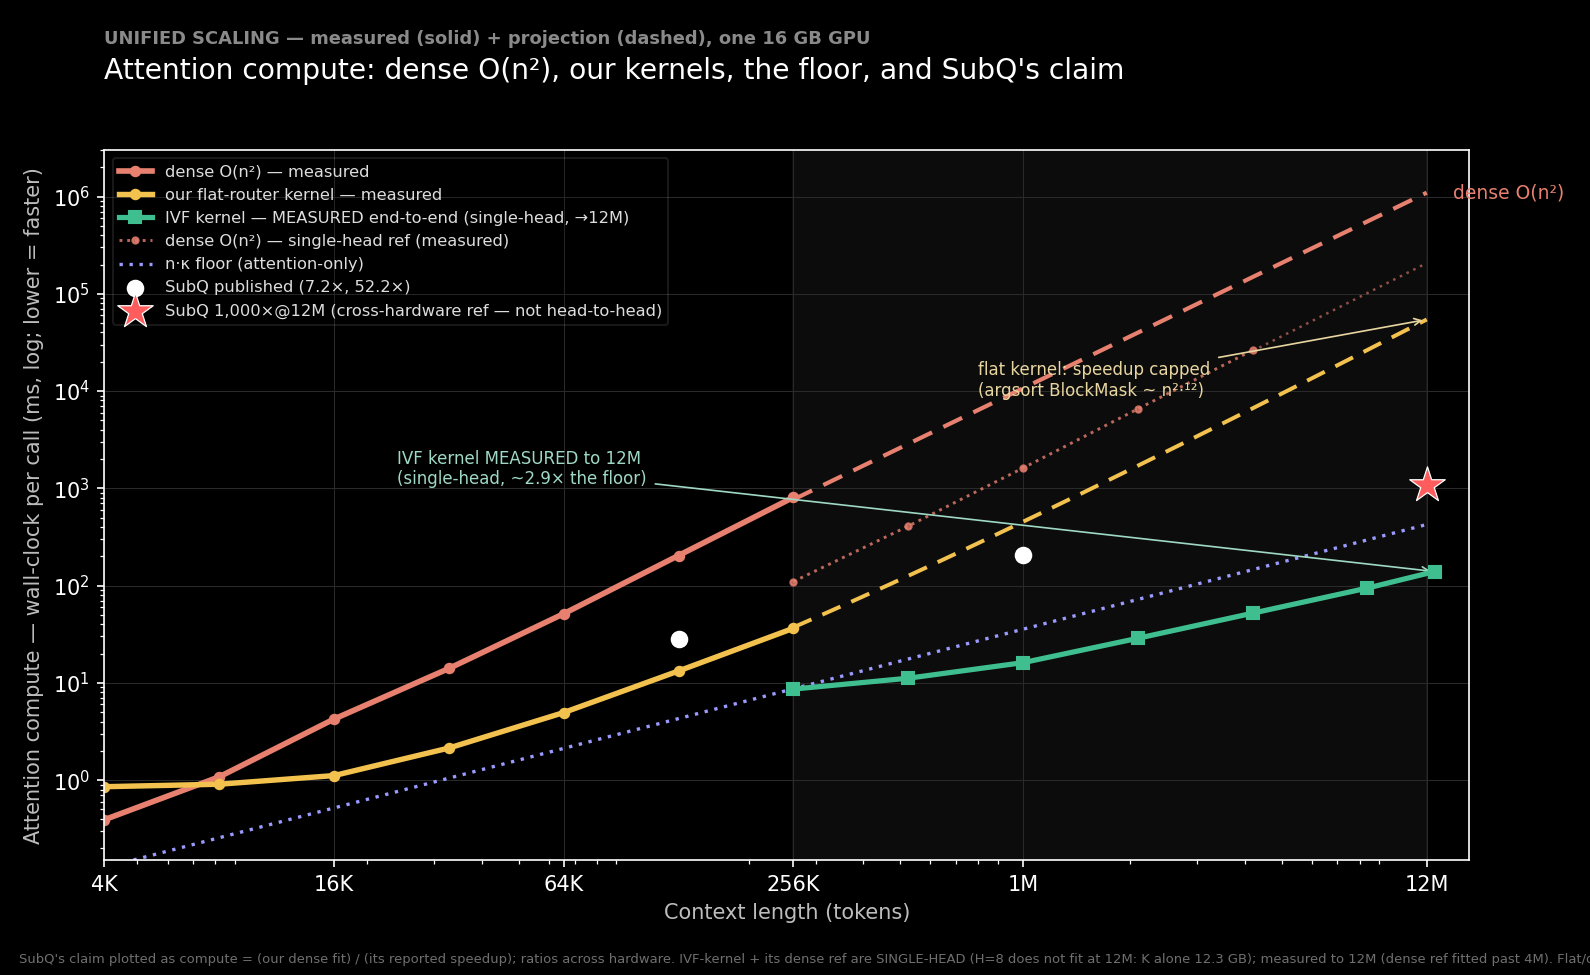
\includegraphics[width=\linewidth]{figures/unified_scaling.png}
  \caption{Attention compute versus context length (lower is faster). Dense $O(n^2)$ rises at the top; our
  flat-router kernel (measured) stays well below it but its speedup is capped because the argsort
  \texttt{BlockMask} build grows nearly as fast; the measured faiss-GPU IVF router drops the kernel onto the
  $n\kappa$ floor. SubQ's two published speedups and its $1{,}000\times$@12M claim are shown as compute
  $=$ dense$/$speedup. Measured solid, projection dashed; one 16\,GB GPU.}
  \label{fig:unified}
\end{figure}

Selection caps the per-query work at a budget $\kappa$ keys, so the irreducible cost of the layer is the
\emph{attention floor} $n\kappa$---linear in $n$. A measured kernel sits above this floor by exactly its
router cost. Decomposing one forward of the kernel of \S\ref{sec:pipeline} into router (the $(n/b)^2$
block-score GEMM), \texttt{BlockMask} construction, and attention, and fitting each over
$n\in[16\mathrm{K},524\mathrm{K}]$, gives attention ${\sim}\,n^{1.02}$ (the floor), router ${\sim}\,n^{1.76}$,
and---largest---the argsort-based mask build ${\sim}\,n^{2.12}$. Extrapolated to $12\mathrm{M}$ tokens the floor
is ${\sim}1\%$ of the forward: a $128\times$ gap, entirely the two $(n/b)^2$ terms. A router that emits the
selected block indices \emph{directly} removes both (Figure~\ref{fig:unified}).

\paragraph{Lowering the floor.} The floor $n\kappa$ itself drops if fewer keys recover the target. The smallest
budget $\kappa_{\min}$ reaching recall $\ge 0.9$ is $\kappa_{\min}/n=3\%$ for tight clusters, $50\%$ for diffuse
or adversarial geometry (no compression), and the routability regularizer of \S\ref{sec:routability} drives it
from $25\%$ ($\lambda=0$) to $\mathbf{0.4\%}$ ($\lambda=64$)---a $60\times$ reduction, the dominant lever, on
benign geometry only.

\paragraph{Closing the gap.} The necessity argument of \S\ref{sec:trilemma} forces a sub-linear, examine-$o(B)$
index. A bake-off on benign co-trained keys (recall vs.\ keys scored) ranks an IVF (inverted-file) router and a
recursive-radius treecode ahead of LSH, which fails to reach recall $0.9$. An IVF over the block means scores
$O(\sqrt{n/b})$ blocks at $0.93$--$0.97$ block-selection agreement with the flat router and emits
\texttt{kv\_idx} directly. Timed on a single 16\,GB GPU with both routers on-device (no host transfer), the
dense $(n/b)^2$ GEMM's constant wins below ${\sim}2\mathrm{M}$ but its score matrix exhausts memory at
$4\mathrm{M}$; the IVF runs linearly past it:

\begin{center}\small
\begin{tabular}{lrrl}
\hline
context $n$ & flat $(n/b)^2$ GEMM & faiss-GPU IVF & winner\\
\hline
256K & $0.21$\,ms & $7.3$\,ms & flat $35\times$\\
2M & $14.0$\,ms & $19.5$\,ms & flat $1.4\times$\\
4M & $52.6$\,ms (runs) & $31.4$\,ms & IVF $1.7\times$\\
8M & OOM ($nb^2{=}17.2$\,GB) & $63.7$\,ms & IVF only\\
\hline
\end{tabular}
\end{center}

\noindent The crossover is ${\sim}3\mathrm{M}$. This stripped single-head GEMM OOMs only at $8\mathrm{M}$
($17$\,GB matrix), while the kernel's \emph{actual} router (\texttt{block\_route}, $H$ heads $+$ an argsort)
OOMs near $1\mathrm{M}$---so the IVF is the only router that runs at long context and is measured to
$12\mathrm{M}$ ($94$\,ms).

\medskip\noindent\textbf{The gap, closed end-to-end (measured).} Wiring the IVF router into the kernel---it
emits the compressed block-index contract directly, and the mask is built without the dense
$(n_b,n_b{+}1)$ transpose (which would need $38.7$\,GB at $n_b{=}98{,}304$)---lets the whole forward be measured,
single-head, to $12\mathrm{M}$ on one $16$\,GB GPU: router $101$\,ms, mask build $0.003$\,ms, attention (the
floor) $47.5$\,ms, \emph{total $139.5$\,ms} in $6.55$\,GB. The direct-index mask build is $0.003$\,ms,
compared with a $40.7$\,s extrapolation for the argsort path, and the residual gap to the floor is a measured
$2.9\times$. The scope is single-head ($H{=}8$ does not fit at $12\mathrm{M}$) and synthetic keys (a speed result),
and the whole result is conditional on benign geometry---adversarial or multi-hop retrieval returns
$\kappa_{\min}$ to the $50\%$ floor, where no speedup exists. Both ingredients of a quality-preserving
large-context speedup---a floor-lowering training stage and a sub-linear indexer---are thus exhibited, and the
indexer is shown driving a live kernel to ${\sim}$the floor, under exactly that benign-geometry condition.

\section{Experiments}\label{sec:experiments}

The evidence below is organized by current claim and fixture. Synthetic timing establishes kernel scaling;
controlled training establishes mechanism behavior; frozen pretrained models establish integration and
retrieval behavior. Only the complete 10M experiment combines real-model geometry, every layer and head,
long context, subquadratic routing, sparse execution, and an observed quality outcome.

\paragraph{Routing.} Second-order (cumulant) routing recovers targets where centroid routing collapses,
matching the $1/b$ outlier-attenuation analysis of Section~\ref{sec:secondorder}; routing quality peaks near
$\beta\approx2$, consistent with the bias--variance reading of~\eqref{eq:lse}.

\paragraph{Kernel speedup.} A block-sparse implementation of Algorithm~1 achieved a $20.6\times$ wall-clock
speedup over a dense exact kernel at $n=262{,}144$ on a single accelerator, with the crossover well below that
length.

\paragraph{The IVF kernel, measured to 12M.} Wiring the sub-linear IVF router into the kernel
(Section~\ref{sec:floor}) and measuring the whole forward single-head on one $16$~GB GPU runs a
\emph{$12$M-token forward in $139$~ms and $6.55$~GB}, at a measured $2.9\times$ the $n\!\cdot\!\kappa$ floor
(versus the $128\times$ gap the flat kernel projected); the argsort mask build collapses to sub-millisecond
because the IVF emits block indices directly. The autoregressive decode step is \emph{flat in $n$}
(${\sim}0.6$~ms from $1$M to $12$M at fixed $\kappa$) while a fair fp16 flash-decode step's prefix read grows
with $n$ ($0.5\to5.3$~ms)---a $9\times$ per-step gap at $12$M with the crossover near $1$M--$2$M, both
measured. The comparison uses the fair fp16 flash-decode row; a naive fp32-upcasting reference remains in the
benchmark only as a diagnostic. This is a single-head synthetic-key speed result; selection quality is a
separate benign-geometry claim.

\paragraph{Multi-hop composition.} A chained retrieval through the same budgeted block selector obeys the
composition law $\text{chain}\approx\prod_j\rho_j$: benign single needles hold at $1.00$ while a \emph{mixed}
two-hop chain (one benign hop, one isolated hop) collapses to $0.02$ at $n=65{,}536$---the isolated hop's
$\rho\!\approx\!0.02$ divides the product. The multi-hop sag is the single-needle result read $h$ times,
reproducing the NIAH${\gg}$MRCR benchmark split as a prediction of the same theory rather than an anomaly.

\paragraph{The fused kernel inside a real model.} Swapping the kernel into a pretrained Qwen2.5-0.5B and
measuring at $8$K--$128$K preserves single-needle NIAH at $1.00$ while giving a $1.5$--$1.6\times$ prefill
speedup at $32$K (budget $0.06$--$0.12$), the speedup growing with $n$ and with a tighter budget---the
synthetic-key crossover shape inside a real model. At matched budget the analytic $O(n^2)$ path needs
$10.7$~GB and $3.5$~s where the fused kernel needs $1.4$~GB and $130$~ms, and the analytic path OOMs before
$64$K while the kernel reaches $128$K (under YaRN). This configuration jointly measures a real model, long
context, a subquadratic kernel, and quality at $0.5$B scale.

\paragraph{Complete pretrained transformer beyond 10M.} The memory-bounded Qwen2.5-0.5B path processes
\emph{$10{,}000{,}128$ tokens} through all 24 layers, 14 query heads, and 2 KV heads on one RTX Pro 6000. It
completes in \emph{$713.2$~s} at \emph{$14{,}022$ token/s} with \emph{$25.72$~GB} peak CUDA allocation. The
fixed-beam center-radius tree routes on pre-RoPE content geometry; native GQA sparse attention scores the
selected blocks with post-RoPE Q/K. Layer-1 cross-head consensus and a bounded 128-block cross-layer reservoir
retain route evidence while keeping the per-query/head budget at no more than 198 blocks, an upper selected
fraction of \emph{$0.506\%$}. The 4K dense-equivalence gate, dense and streamed 128K NIAH gates, and the 10M
semantic ranking pass (\texttt{walnut} 5.844, best distractor 4.438). The model is frozen and uses static YaRN
at approximately $306\times$ its training range. Consequently this experiment demonstrates the full execution
conjunction and one successful quality outcome, not dense-equivalent output or general long-context quality.

\paragraph{An optimal selector: the Certified Causal Cascade.} Composing five ingredients---a shared low-dim
routing space, sub-block max-pool summaries, a chunked-causal streaming index, an exact outlier side-channel,
and per-query admissible certificates with escalation---into one streaming selector. The certificate is sound
(certified $\Rightarrow$ the selected blocks equal the parent-index-tie-broken top-$\kappa$ under the routing
metric; zero violations on clustered and random geometry). In the indexed regime its skip and truncation
checks are strict at the returned threshold; an exhaustive tie instead follows the explicit index policy.
This certifies the routing metric, not the omitted
softmax mass or attention-output error; the latter have a separate reference certificate in
Section~\ref{sec:output-cert}. The component table is the trilemma made concrete:
sub-block granularity and the outlier channel rescue high-norm spikes, but \emph{isolated unit-norm needles
stayed unretrievable for every tested cheap selector} (recall $0.05$)---the grounded-probe obstruction of
Section~\ref{sec:trilemma} in miniature, not an unrestricted indexing lower bound. Per-layer routing is
${\sim}59\%$ of a Qwen-0.5B prefill (at DSA's reported $58\%$), and
the lever that makes it cheap is \textbf{cross-layer sharing from a mid donor layer}---measured cutting it to
${\sim}6\%$ with single-needle retrieval preserved, consistent with the analytic $\div 5$ estimate; sharing
from layer~0 fails. A trained $d_r{=}16$ projection reaches $0.65$ block agreement on real keys versus $0.32$
untrained, but is itself too lossy to drive retrieval---the honest boundary.

\paragraph{The compression corner, measured.} The trilemma has a second corner---a fixed- or growing-state
memory written at inference time (the ``zero attention'' / DeltaNet/Titans family). Small exact reference
memories, measured against Lean predictions, place it. The READ rule sets the capacity class: a linear read
$o = S q$ is rank-$d$ capped (recall collapses at $m\approx d$; \texttt{read\_capacity\_le\_dim} /
\texttt{rank\_d\_read\_wall} prove the $\le d$ ceiling) while a softmax read over the same pairs holds
far past $m=d$ (measured to $m=512$; \texttt{softmax\_capacity} gives the exponential form)---capacity is a
property of the read, not the substrate, with machine-checked results on both sides of the contrast. The load-bearing measurement (empirical, no theorem) is that
\textbf{compression $\neq$ selection}: a needle salient only at read time is lost by a surprise-gated fixed
memory (recall $0.10$) where selection recovers it ($1.00$)---write-time compression cannot keep what the future
query has not yet made relevant. A distribution shift is a fold a fixed memory cannot track
(\texttt{fold\_not\_hopfield}: pre-shift recall decays $0.90\to0.10$; a growing slot-birth state holds $0.65$),
and the proved composition bound $\prod\rho \le \min$-hop (\texttt{chain\_le\_weakest}) is reproduced, the
measured joint chain sagging below $\prod\rho$. The NIAH-$\gg$-multi-hop split is thus architecture-independent
---it holds whichever corner of the trilemma one builds.

\paragraph{The compression corner, trained.} The reference memories above are untrained; the zero-attention
recipe's load-bearing half is \emph{training-dependent}---a learned write gate and an auxiliary
future-prediction objective. The trained fixture is a small micro-LM ($d=128$, head dimension $d_h=16$) trained
end-to-end on MQAR with a token-mixer swappable between the two corners at matched state (DeltaNet state $d_h$
vs.\ an SSA budget $\kappa\approx d_h$). Three measurements. (i)~\emph{Capacity:} trained selection (dense, SSA)
is flat in load, while the trained DeltaNet groks the task and holds to $m\approx d_h$ then walls at the same
rank-$d_h$ boundary---training moves the wall, it does not remove it. (ii)~\emph{The learned write gate has no
measured benefit:} on write-salient MQAR (keep-worthy pairs use reserved marker keys, identifiable at write
time) the no-gate delta rule already solves it---training shapes the $\le d_h$ keepable keys itself; on
read-salient MQAR nothing lifts the compression wall, gate or no gate. (iii)~\emph{The future-prediction
auxiliary loss is flat in its weight} on the read-salient wall. So the training-dependent half of the recipe
does not close the gap: where keeping is possible training already does it, and where relevance is
read-time-only no write policy can serve it---the trained mirror of the $0.10$-vs-$1.00$ split, and the
composition sag persists for the compression corner under training as well. The bottom line: dropping attention
does not dissolve the trilemma but relocates within it---a compression memory \emph{works} where relevance is
fixed at write time and within its state (write-salient recall, NIAH), and \emph{fails}, by capacity rather
than by any trainable objective, on read-time-only relevance, past-capacity retrieval, and multi-hop chains.
This is why the frontier long-context state-space models remain \emph{hybrids} with interleaved attention.

\paragraph{Routability.} The regularizer~\eqref{eq:reg} reduced lossless branch-and-bound selection cost from
$26.5\%$ to $4.2\%$ of keys. (Accuracy is $1.000$ by construction---admissible-bound branch-and-bound always
returns the exact argmax---so the measured quantity is the \emph{cost}, not task accuracy.) The reduction was
robust across head dimension; the capacity--search tension is a genuine asymptotic trade-off, but it did not
bite for $d\ge$ (number of clusters), since query-specific anisotropy needs only ${\sim}1$ dimension per
cluster---real head dimensions ($64$--$256$) sit above this, the trade reappearing only as $d\to$ (number of clusters).

\paragraph{Length generalization and staging.} See Section~\ref{sec:length}: $32\times$ the trained length at
recall $0.982$ for ${\sim}800$ adaptation steps, SSA-preserved.

\paragraph{Construction pipeline.} See Section~\ref{sec:pipeline}: swap $+13.2$ perplexity, $94\%$ recovered to
within $+1.2$ of the dense-adapted control at ${\sim}38\%$ of keys.

\paragraph{Real-model frozen-swap (Gemma-4-26B).} Beyond the $124$M control, the swap-and-route was
validated end-to-end on a frozen \emph{Gemma-4-26B-A4B} (mixture-of-experts, $4$B active): SSA was installed
into its five full-attention layers (head dimension $512$, $K{=}V$, grouped-query) via the attention
interface and scored on needle-in-a-haystack retrieval against the selection budget at $n=2048$. Plain
second-order (cumulant) routing recovers retrieval down to a $50\%$ budget (recall $1.00$) but collapses at
$25\%$ (recall $0.00$); a forward-only probe shows the distant needle's block ranks ${\approx}3$rd by the
cumulant score---just outside the kept top-$2$---and worst at the deepest layer, a position-decay effect.
Adding the third-cumulant (skew) term of the tempered family (Section~\ref{sec:secondorder}) restores the
$50\%$ budget to $1.00$ and lifts the $25\%$ budget to $0.44$ (to $0.56$ if the single worst-routing layer is
left dense). This residual is a \emph{tuning artifact}, not a frozen-key ceiling: at a finer block size,
plain second-order routing reaches recall $1.00$ at the $25\%$ budget---the third-cumulant term is a
coarse-block compensator, unnecessary (and at large $\beta$ harmful) once the needle dominates a small block.
So at moderate $n$ the frozen model retrieves fully under the right routing granularity; key co-adaptation
(the routability regularizer, \eqref{eq:reg}) is for the long-context regime, where the block-score
computation itself becomes quadratic. This is a routing-\emph{quality} measurement (the analytic,
score-materializing swap at moderate $n$), not the subquadratic-kernel regime. The routing survives a
doubling of context---a forward-only probe shows the far needle staying within the $25\%$ budget from $n=2048$
to $n=4096$, carried by a stable subset of layers. This remains an analytic routing-quality result with no
Gemma speed claim. The separate Qwen experiment above supplies complete real-model execution evidence beyond
10M; it does not extend the Gemma result to that length.

\paragraph{Retrieval regime boundaries.} The complete 10M run supplies one successful semantic ranking. The
controlled sweep below isolates the geometry behind such single-target results by measuring retrieval as a
function of context length at fixed budget $\kappa\approx10^3$ and margin $\Delta=0.55$:

\begin{center}
\begin{tabular}{@{}rccc@{}}
\toprule
context $n$ & dense & SSA, isolated target & SSA, benign target\\
\midrule
1024   & 1.00 & 1.00 & 1.00\\
4096   & 1.00 & 0.47 & 1.00\\
16384  & 1.00 & 0.20 & 1.00\\
65536  & 0.90 & 0.10 & 1.00\\
262144 & 0.83 & 0.00 & 1.00\\
\bottomrule
\end{tabular}
\end{center}

An \emph{isolated} target---a lone spike with no correlated neighbors---\emph{collapses} with length: cheap
moment routing averages it into its block and loses it among the fluctuations of the growing number of blocks
(the $1/b$ attenuation of Section~\ref{sec:secondorder}, competing against more and more random blocks).
This is Proposition~\ref{prop:impossible} in miniature. A \emph{benign} target---one accompanied by a coherent
span of query-aligned neighbors, as a real answer is by its surrounding context---lifts its whole block's score
and stays flat at $1.00$, \emph{beating dense} at long $n$ because selection caps the effective distractor
count. The same separation appears across margins: an isolated target barely fires at any margin, while a
benign one tracks dense once the margin clears the budget floor $\sqrt{2\log\kappa/d}$. So the headline numbers
certify the \emph{easy and benign} regime (single, high-margin, accuracy not losslessness)---the regime
everyone agrees is achievable---and do not certify lossless selection in the worst case, which
Proposition~\ref{prop:impossible} shows is unavailable cheaply.

\section{Discussion and limitations}

SSA is best understood as the resolution of a constrained problem rather than a universal accelerator. The
recovery-weight law~\eqref{eq:recovery} shows selection makes retrieval flat in $n$; the admissible
bound~\eqref{eq:admissible} and the prune gate~\eqref{eq:prune} show summaries can certify that selection
losslessly; the trilemma (Section~\ref{sec:trilemma}) shows this can be cheap \emph{only} on benign geometry;
and the regularizer~\eqref{eq:reg} shows training can supply that geometry. The construction pipeline
(Section~\ref{sec:pipeline}) and the staging ladder (Section~\ref{sec:length}) turn the mechanism into a recipe
that retrofits a dense model and extends its context a rung at a time.

The current limitations follow directly from the theory and evidence. (i)~\emph{Worst-case losslessness is not available cheaply}
---a sufficiently adversarial or genuinely low-margin target can always evade summary routing; SSA's guarantees
are conditional on the (trained, measured) benign geometry. (ii)~\emph{Multi-needle and low-margin retrieval}
are the hard regime the headline single-needle numbers do not address. (iii)~The selection budget $\kappa$ sets
a floor margin $\sqrt{2\log\kappa/d}$; targets below it are missed regardless of $n$. (iv)~The complete 10M
experiment uses a frozen 0.5B model, static YaRN far outside its training range, one semantic NIAH ranking,
and no dense 10M baseline; it is execution evidence rather than a broad quality result. (v)~The 12M IVF
near-floor timing is single-head and synthetic, while the real-model 128K timing and quality measurements are
smaller-scale. Broad retrieval, perplexity, multi-hop evaluation, trained long-context models, and
frontier-model validation remain open. (vi)~The complete implementation is not formally verified end to end.
Appendix~\ref{app:invariants} gives self-contained statements and proofs of the supporting exact-arithmetic
invariants; access to the separate formalization is not required to inspect them. As corroborating provenance,
private Substrate commits from the potential-store precursor \texttt{88a4c7012} through
\texttt{fad55ff82} machine-check the corresponding results for
recursive real-valued ball containment and monotone drop sets, causal prefix-cut selection, conditional
9-vote retention by a 128-slot highest-count reservoir at the 14-selector/70-item route bounds, and survival
with a uniform cardinality cap under union with a fixed carrier. It also checks the structural two-pass
comparison and its fixed-pass expressivity fence, the strictly-causal finite-transfer identity, and the RoPE
winding facts stated below.
It also proves that the radial pairing cap is attained under alignment plus a realizable boundary member and
that the per-centre refinement agrees there. Those alignment hypotheses are sufficient, not shown necessary.
The per-centre cap is universally no larger; a plane witness exhibits a strict gap as large as the whole cap,
but no converse says nonalignment forces strictness or equality forces alignment. These results do not
formally verify the Python/CUDA mapping, float32 outward rounding, fixed-beam quality, or the unrecorded
premise that the measured target had nine pre-consensus base-route votes. The float32 portion is instead
addressed experimentally below.

That audit also closes four previously separate proof obligations. First, the restricted-read TV, KL, exact
output residual, two block-output bounds, equal-value fence, and smoothed reverse-divergence limit are one
checked family. Second, admissible region caps plus strict skip and truncation tests return the strict top set;
without strict separation, an explicit index order is needed to name one set. SSA now breaks exact parent-score
ties by the larger parent index. Third, the adaptive read-budget ceiling is the grounded-probe theorem stated
in Section~\ref{sec:trilemma}, including its finite-randomized extension and zero-depth counterexample. Fourth,
the nine-vote retention, fixed-carrier union, \texttt{roundWidth + 128} capacity, past bound, and causal cut are
checked as one composed routing plan. The last statement is still conditional on the vote floor and says
nothing about attention-output quality, FLOPs, or latency.

The newer formal layer connects those routing facts to a finite score/value store whose softmax read is the
derivative of its log-partition and proves the exact append law~\eqref{eq:append-read}. It turns the
mean/variance routing statistic into the bounded-range interval~\eqref{eq:cumulant-interval}, while explicitly
requiring third-cumulant control along the whole tilt segment. It composes state-dependent routed-read errors
by the Lipschitz recurrence~\eqref{eq:sequential-error}, with a counterexample ruling out a final bound from
local error alone. It also proves that the pointwise query-group pairing maximum is the least shared safe
claim and is invariant under one common isometry, defines the distribution-weighted node-read objective and
finite certified-partition choice, and extends the single-spike read ceiling to finite-state indexed and
finite-randomized readers. None of these results constructs a cheap summary, learns a partition, supplies the
required Lipschitz constants, proves route quality, or turns finite state count into an implementation cost.

The variance-sensitive extension proves~\eqref{eq:bennettmass}, lifts it through trace spread, arbitrary tree
frontiers, causal cuts, and the omitted-mass/output certificate, and gives conditional node/key work counts.
Its later full-covariance identity makes $q^TCq$ the exact directional variance with no dimension factor. The
resulting subquadratic statement still assumes a bounded active frontier and the arithmetic work inequality;
the Qwen measurement above shows neither trace nor full covariance establishes that premise on the tested
tree. The outlier-peel extension proves the order-statistic and recentring radii,
exact-exposed-plus-core cap, running-minimum/frontier/causal/output transport, and conditional $O(td)$
work/storage accounting. It does not prove that any fixed peel depth makes the active frontier bounded. Its
Inference consumer re-exports these facts without weakening their premises: residual moments and radii are
supplied, while subquadraticity still requires bounded active width, the stated certificate charge, and the
explicit total-work inequality.

The production tree inflates every recursive norm-plus-child-radius result by
$8(d+4)\varepsilon_{32}$ and rounds the candidate and selected maximum toward $+\infty$; query/node score
caps receive an analogous absolute-error allowance and upward final rounding. On an RTX 4080, the public
verifier compared the actual tree with float64 descendant oracles across five ordinary and adversarial
geometries and fanouts 2, 4, and 16. Unguarded arithmetic underestimated 8,701 of 90,105 radii and 367,480 of
1,081,260 score caps. The guarded implementation had zero observed underestimates. At 65,536 leaves,
dimension 64, and fanout 16, construction measured 0.433 ms guarded versus 0.223 ms raw. This is empirical
stress evidence, not a directed-rounding proof, and it does not turn the fixed-beam traversal into exact
top-$k$ search. The complete record is \texttt{runs/float\_tree\_verification.json}; reproduce it with
\texttt{python -m ssa.float\_tree\_verification}.

Two adjacent results remain boundaries rather than implementation claims. A positive log-concave score-spread
function has a nonincreasing ratio across any fixed nonnegative displacement, but SSA has not established that
empirical hypothesis and the result is not an admissible skip bound. Separately, for a strictly
below-diagonal linear interaction $A$ on an $n$-position carrier, $A^n=0$ and
$(I-A)^{-1}=\sum_{k=0}^{n-1}A^k$ without a decay condition. Ordinary causal softmax includes its diagonal and
a transformer includes nonlinear stages, so this identity does not make one SSA layer a complete multi-hop
solver; it clarifies why the measured two-hop failures remain an empirical model-and-routing question.

The compression comparator has a separate sign boundary. A product of gains in $[0,1]$ can shrink or erase a
stored scalar but cannot reverse its sign; once negative gains are admitted, reversal is determined by their
parity. For the DeltaNet-style rank-one correction $T(x)=x-\beta\inner{k}{x}k$, the key direction has gain
$1-\beta\lVert k\rVert^2$ and becomes the exact reflection across $k^\perp$ at
$\beta\lVert k\rVert^2=2$. This explains a capability boundary of the compression arm; it does not improve or
certify SSA's selector.

\appendix
\section{Derivations}

\paragraph{A.1 Recovery weight~\eqref{eq:recovery}.} With one target at logit $a_\star$ and $\mu$ distractors
at $a_\star-\Delta$, $w_\star=e^{\beta a_\star}/(e^{\beta a_\star}+\mu e^{\beta(a_\star-\Delta)})$. Divide
numerator and denominator by $e^{\beta a_\star}$ to get $1/(1+\mu e^{-\beta\Delta})=\sigma(\beta\Delta-\log\mu)$,
since $1/(1+e^{-x})=\sigma(x)$ with $x=\beta\Delta-\log\mu$.

\paragraph{A.2 Cumulant score~\eqref{eq:route}.} Let $g(\beta)=\beta^{-1}\log\frac1b\sum_{j\in
c}e^{\beta\inner{q}{k_j}}$. As $\beta\to0$, $g(\beta)=\E_j\inner{q}{k_j}+\frac{\beta}{2}\Var_j\inner{q}{k_j}
+O(\beta^2)$, the cumulant generating function expansion. The mean is $\inner{q}{\mu_c}$ and the variance is
$q^\top\Sigma_c q$, giving~\eqref{eq:route}.

\paragraph{A.3 Log-sum-exp sandwich~\eqref{eq:lse}.} For any reals $x_1,\dots,x_b$ with $M=\max_j x_j$:
$e^{\beta M}\le\sum_j e^{\beta x_j}\le b\,e^{\beta M}$. Take $\log$, divide by $\beta$:
$M\le\beta^{-1}\log\sum_j e^{\beta x_j}\le M+\beta^{-1}\log b$.

\paragraph{A.4 Samuelson bound~\eqref{eq:samuelson}.} Center the data, $d_j=s_j-\bar s$, so $\sum_j d_j=0$. Fix
index $i$. By Cauchy--Schwarz over the other $m-1$ indices,
$d_i^2=(\sum_{j\neq i}d_j)^2\le(m-1)\sum_{j\neq i}d_j^2=(m-1)(\sum_j d_j^2-d_i^2)$. Hence $d_i^2\,m\le(m-1)\sum_j
d_j^2$, i.e.\ $(s_i-\bar s)^2\le(m-1)\Var$. Taking the max over $i$ and adding $\bar s$ gives the stated bound on
$\max_j s_j$, and~\eqref{eq:prune} is its contrapositive against the threshold $s^\star$.

\setcounter{proposition}{0}
\renewcommand{\theproposition}{B.\arabic{proposition}}
\renewcommand{\theHproposition}{B.\arabic{proposition}}
\section{Self-contained routing invariants}\label{app:invariants}

This appendix contains the mathematical content used to justify the 10M router's center-radius hierarchy,
bounded top selection, adaptive read-budget boundary, causal selected reads, cross-head reservoir, fixed
cross-layer carrier, finite potential and append laws, cumulant intervals, sequential error composition,
query-group transport, distribution-weighted safe partitions, finite index capacity, and the
variance-sensitive mass tree, plus the factorized-attention and strictly-causal comparisons used to delimit
the claims.
The restricted-read/output proof is already self-contained in Section~\ref{sec:output-cert}. It is included so
the public artifact does not depend on access to the separate Lean repository. The formal audit is useful
corroboration, but the definitions,
statements, proofs, counterexamples, and scope needed to assess the claims are all below. Every geometric
statement is over an exact real inner-product space. The production implementation uses conservative
outward inflation and is stress-tested against float64 oracles as reported above; that experiment is not a
proof of all floating-point executions.

\subsection{Finite families of key regions}

Let $I$ be finite and nonempty. In a real inner-product space, let key $x_i$ lie in the closed ball with centre
$c_i$ and radius $r_i$:
\[
\lVert x_i-c_i\rVert\le r_i .
\]
For a reference point $p$, define the \emph{radial reach} and its score cap by
\begin{equation}\label{eq:app-reach}
R=\max_{i\in I}\bigl(\lVert c_i-p\rVert+r_i\bigr),
\qquad U_R(q)=\inner{q}{p}+\lVert q\rVert R .
\end{equation}

\begin{proposition}[Admissibility and radial minimality]\label{prop:app-radial}
For every $i$ and $q$,
\[
\lVert x_i-p\rVert\le R,
\qquad \inner{q}{x_i}\le U_R(q).
\]
Moreover, $R$ is attained by some index and is the least number satisfying
$\lVert c_i-p\rVert+r_i\le R$ for all $i$.
\end{proposition}
\begin{proof}
The triangle inequality gives
\[
\lVert x_i-p\rVert
\le \lVert x_i-c_i\rVert+\lVert c_i-p\rVert
\le r_i+\lVert c_i-p\rVert\le R.
\]
Then
$\inner{q}{x_i}-\inner{q}{p}=\inner{q}{x_i-p}
\le\lVert q\rVert\lVert x_i-p\rVert\le\lVert q\rVert R$
by Cauchy--Schwarz. Attainment and minimality follow directly because~\eqref{eq:app-reach} is the maximum of a
finite, nonempty family.
\end{proof}

Radial minimality does \emph{not} make $U_R$ the sharpest score bound available from the same data. Define the
per-centre cap
\begin{equation}\label{eq:app-per-centre}
U_C(q)=\max_{i\in I}\bigl(\inner{q}{c_i}+\lVert q\rVert r_i\bigr).
\end{equation}

\begin{proposition}[Per-centre refinement]\label{prop:app-per-centre}
Every key is bounded by its own centre,
\[
\inner{q}{x_i}\le\inner{q}{c_i}+\lVert q\rVert r_i,
\]
and $U_C(q)\le U_R(q)$ for every query.
\end{proposition}
\begin{proof}
Apply Cauchy--Schwarz to $x_i-c_i$ for the first inequality. For the second, apply it to $c_i-p$:
\[
\inner{q}{c_i}+\lVert q\rVert r_i
\le \inner{q}{p}+\lVert q\rVert
   \bigl(\lVert c_i-p\rVert+r_i\bigr)
\le U_R(q),
\]
then maximize the left side over $i$.
\end{proof}

The comparison can be strict. In $\R^2$, take one region with $p=(0,0)$, $q=(1,0)$,
$c_1=(0,1)$, $r_1=0$, and $x_1=c_1$. Then $R=1$ and $U_R(q)=1$, whereas
$U_C(q)=\inner{q}{x_1}=0$. Thus the gap can equal the whole reach term. This is one witness, not a
theorem that nonalignment always makes the inequality strict.

For the equality case, write $e_q=\lVert q\rVert^{-1}q$, using $e_0=0$. Say two vectors are on the same ray
when one is a nonnegative scalar multiple of the other; then
$\inner{q}{v}=\lVert q\rVert\lVert v\rVert$.

\begin{proposition}[Aligned realizable attainment]\label{prop:app-attainment}
Suppose an index $i_\star$ attains the reach,
$\lVert c_{i_\star}-p\rVert+r_{i_\star}=R$, the vectors $q$ and $c_{i_\star}-p$ lie on the same ray, and
\begin{equation}\label{eq:app-boundary}
x_{i_\star}=c_{i_\star}+r_{i_\star}e_q .
\end{equation}
Then
\[
\inner{q}{x_{i_\star}}=U_R(q).
\]
Consequently, if $B$ bounds every $\inner{q}{x_i}$ for this fixed family and query, then
$U_R(q)\le B$; no smaller skip bound is admissible there. Under the reach-attainment and same-ray hypotheses
alone---without the boundary-member hypothesis~\eqref{eq:app-boundary}---$U_C(q)=U_R(q)$.
\end{proposition}
\begin{proof}
Same-ray equality and~\eqref{eq:app-boundary} give
\[
\begin{aligned}
\inner{q}{x_{i_\star}}
 &=\inner{q}{p}+\inner{q}{c_{i_\star}-p}
   +r_{i_\star}\inner{q}{e_q}\\
 &=\inner{q}{p}+\lVert q\rVert
   \bigl(\lVert c_{i_\star}-p\rVert+r_{i_\star}\bigr)=U_R(q).
\end{aligned}
\]
Any common bound $B$ must bound this member, proving the next claim. For the cap comparison, the
$i_\star$ term in~\eqref{eq:app-per-centre} equals $U_R(q)$ under alignment, while
Proposition~\ref{prop:app-per-centre} supplies the reverse inequality.
\end{proof}

No $q\ne0$ hypothesis is needed: at $q=0$, $e_q=0$ and both sides vanish. Nor does equality require
$r_{i_\star}\ge0$. That sign condition is needed only to make the constructed boundary member admissible:
$\lVert r_{i_\star}e_q\rVert\le r_{i_\star}$ when $r_{i_\star}\ge0$. The hypotheses above are sufficient;
neither attainment nor equality of the two caps is proved to force alignment.

\subsection{Recursive ball containment}

Define a ball tree recursively. A leaf stores a centre and radius. A node stores a centre $c_t$ and children
$u$, and its radius is
\begin{equation}\label{eq:app-tree-radius}
\rho_t=\max\!\left(0,\max_{u\text{ child of }t}
  \bigl(\lVert c_u-c_t\rVert+\rho_u\bigr)\right).
\end{equation}
Let $s\preceq t$ mean that $s=t$ or $s$ is below $t$ through a finite chain of child edges.

\begin{proposition}[Containment and ancestor cap]\label{prop:app-tree}
Every child ball lies inside its parent ball. More generally, if $s\preceq t$ and
$\lVert x-c_s\rVert\le\rho_s$, then
\[
\lVert x-c_t\rVert\le\rho_t.
\]
For every reference point $p$, ancestor reach is monotone:
\[
\lVert c_s-p\rVert+\rho_s
\le \lVert c_t-p\rVert+\rho_t.
\]
Consequently, if each key lies in a descendant ball below $t$ and
$\lVert c_t-p\rVert+\rho_t\le R_t$, then
\[
\inner{q}{x_i}\le\inner{q}{p}+\lVert q\rVert R_t
\]
for every such key.
\end{proposition}
\begin{proof}
Equation~\eqref{eq:app-tree-radius} directly gives
$\lVert c_u-c_t\rVert+\rho_u\le\rho_t$ for each child. If $x$ lies in $u$, the triangle inequality yields
$\lVert x-c_t\rVert\le\lVert x-c_u\rVert+\lVert c_u-c_t\rVert\le\rho_t$.
Induction on the child path proves containment. The same induction, now applying the triangle inequality to
$c_u-p$, proves ancestor-reach monotonicity. Proposition~\ref{prop:app-radial} applied at node $t$ gives the
score cap.
\end{proof}

For a fixed query and reference point, write
$U_v=\inner{q}{p}+\lVert q\rVert(\lVert c_v-p\rVert+\rho_v)$. Ancestor-reach monotonicity gives
$U_s\le U_t$ whenever $s\preceq t$. Hence, at every threshold $\theta$,
\[
U_t\le\theta\quad\Longrightarrow\quad U_s\le\theta.
\]
For any finite family of paired ancestor/descendant regions, the descendant drop set therefore contains the
ancestor drop set and has at least its cardinality. Likewise Proposition~\ref{prop:app-per-centre} implies that
the per-centre cap drops every region the reach cap drops. These are consequences of bound dominance at a
fixed threshold; they do not count keys, traversed nodes, or elapsed work.

This establishes exact-real containment at arbitrary depth. It proves neither that a node radius is minimal
nor that the fixed-beam search visits the correct branch. In float32, containment additionally requires radii
to be rounded outward or inflated enough to cover accumulated error. The implementation applies the guard
measured above at every recursive level and to every score cap; zero observed oracle misses do not promote
that guard to a universal arithmetic theorem.

\subsection{Uniform and position-dependent orthogonal actions}

\begin{proposition}[What orthogonality preserves]\label{prop:app-orthogonal}
If one orthogonal map $A$ is applied to the query and both keys, then
\[
\inner{Aq}{Ax}<\inner{Aq}{Ay}
\quad\Longleftrightarrow\quad
\inner{q}{x}<\inner{q}{y}.
\]
Different maps at different key positions need not preserve the order.
\end{proposition}
\begin{proof}
Orthogonality gives $\inner{Au}{Av}=\inner{u}{v}$. For the negative statement in $\R^2$, take
$q=x=(1,0)$, $y=(1/2,0)$, $A=-I$, and $B=I$. Initially
$\inner{q}{y}=1/2<1=\inner{q}{x}$, but
$\inner{q}{Ax}=-1<1/2=\inner{q}{By}$.
\end{proof}

RoPE is position-dependent, so the second statement explains why pre-RoPE and post-RoPE rankings are not
identities. It is only an existence counterexample: it says nothing about how often rankings change or which
ranking gives better retrieval quality.

\subsection{Cross-head consensus and top-count retention}

Let $H$ selectors choose finite sets $S_h$, each of cardinality at most $W$. Let
$U=\bigcup_h S_h$, let $\nu(a)=|\{h:a\in S_h\}|$, and define
$C_v=\{a\in U:\nu(a)\ge v\}$.

\begin{proposition}[Consensus counting]\label{prop:app-consensus-count}
For every $v$,
\[
|C_v|v\le HW,
\]
and for $v>0$, $|C_v|\le\lfloor HW/v\rfloor$.
\end{proposition}
\begin{proof}
Double-count selector--element incidences:
\[
\sum_h|S_h|=\sum_{a\in U}\nu(a).
\]
The left side is at most $HW$, while elements of $C_v$ contribute at least $|C_v|v$ to the right side.
\end{proof}

A \emph{top-count reservoir} of capacity $k$ is a set $T\subseteq U$ such that
$|T|=\min(k,|U|)$ and every outsider has count no larger than every member:
\begin{equation}\label{eq:app-reservoir}
a\in U\setminus T,\ b\in T\quad\Longrightarrow\quad\nu(a)\le\nu(b).
\end{equation}
Such a reservoir exists by sorting the finite pool by $\nu$; ties may be broken arbitrarily.

\begin{proposition}[Consensus retention]\label{prop:app-consensus-retention}
If $v>0$ and $\lfloor HW/v\rfloor\le k$, then every top-count reservoir of capacity $k$ contains $C_v$.
\end{proposition}
\begin{proof}
Suppose $a\in C_v\setminus T$. By~\eqref{eq:app-reservoir}, every $b\in T$ has
$\nu(b)\ge\nu(a)\ge v$, so $T\cup\{a\}\subseteq C_v$. Hence
$|T|+1\le|C_v|\le\lfloor HW/v\rfloor\le k$, giving $|T|<k$. The fullness condition
$|T|=\min(k,|U|)$ then forces $|T|=|U|$. Since $T\subseteq U$, this implies $T=U$, contradicting
$a\notin T$.
\end{proof}

For SSA's route limits, $H=14$, $W=70$, and $v=9$, so
\[
|C_9|\le\left\lfloor\frac{14\cdot70}{9}\right\rfloor=108<128.
\]
Therefore every nine-vote item is retained by any full 128-slot highest-count reservoir, independent of tie
breaking. This is conditional on the item actually receiving nine \emph{pre-reservoir} selections. It says
nothing about items at the implementation's two-vote admission threshold, for which the same bound is
$\lfloor980/2\rfloor=490$.

The fullness equality in the reservoir definition is essential: merely requiring $|T|\le k$ allows the empty
set, which retains nothing. The multiplied counting bound is attained in general when all $H$ selectors choose
the same $W$ items and $v=H$. No construction here is claimed to attain the numeric ceiling 108 at
$(H,W,v)=(14,70,9)$.

\subsection{Accumulating runs and a fixed cross-layer carrier}

Let $S_\ell$ be the selection made at round (or layer) $\ell$, and let $P$ be a carried finite set. There are
two different constructions:
\begin{equation}\label{eq:app-runs}
A_0=P,\qquad A_{n+1}=S_n\cup A_n,
\qquad\text{and}\qquad
F_\ell=S_\ell\cup P.
\end{equation}

\begin{proposition}[Retention and capacity]\label{prop:app-carrier}
The accumulating run satisfies
\[
A_n=P\cup\bigcup_{\ell<n}S_\ell,
\qquad A_n\subseteq A_m\ (n\le m),
\qquad |A_n|\le|P|+nW
\]
when $|S_\ell|\le W$. If additionally $|P|\le C$, the fixed-carrier state satisfies, for every $\ell$,
\[
P\subseteq F_\ell,
\qquad |F_\ell|\le W+C.
\]
\end{proposition}
\begin{proof}
The closed form and monotonicity follow by induction from~\eqref{eq:app-runs}. The cardinality claims use
$|A\cup B|\le|A|+|B|$, once per induction step for $A_n$ and once directly for $F_\ell$. The fixed-carrier
inclusion is immediate from the union.
\end{proof}

The constructions must not be conflated. With $P=\varnothing$ and $S_\ell=\{\ell\}$,
$F_0=\{0\}$ is not a subset of $F_1=\{1\}$, while $A_1=\{0\}\ne F_1$. Thus the fixed carrier preserves
$P$, not every earlier layer's transient selection, and its $W+C$ cap is uniform precisely because it does not
accumulate those selections.

Finally, if ``past-bounded at $t$'' means every member of a set is at most $t$, a union is past-bounded only
when both components are. This property is preserved by either construction under the corresponding
hypotheses; the union does not create it: at $t=0$, $P=\{0\}$ is past-bounded but $S_0=\{5\}$ and
$S_0\cup P$ are not. None of these set identities specifies how a selector admits an item, proves a causal
mask, or proves that the measured target belonged to $P$.

Combining consensus retention, the fixed-carrier bound, and the position cut gives the concrete composed
plan used by SSA. If 14 heads each select at most 70 blocks, $P$ is a full highest-count reservoir of capacity
128, every later selection $S_\ell$ has size at most \texttt{roundWidth}, and both $P$ and $S_\ell$ lie at or
before the query position, then every nine-vote block lies in $P$ and in $S_\ell\cup P$; that union has size
at most \texttt{roundWidth + 128}, remains past-bounded, and its position-cut read is causal. This conjunction
is conditional on the nine-vote premise. A 140-block pooled family in which every block has at most two votes
shows that a full 128-slot reservoir can drop a below-threshold block; capacity alone does not supply the
premise.

\subsection{Selected reads and position causality}

Let $L$ be linearly ordered and let $S\subseteq L$ be a finite routed set. Define the whole-set and
position-cut reads
\begin{equation}\label{eq:app-causal-cut}
W_S(i)=S,
\qquad C_S(i)=\{j\in S:j\le i\}.
\end{equation}
Call a read $R$ causal when $j\in R(i)$ always implies $j\le i$.

\begin{proposition}[Causal cut and composition]\label{prop:app-causal-cut}
The cut read $C_S$ is causal for every $S$. The whole-set read $W_S$ is non-causal whenever some selected
$j$ lies after a query $i$; in particular, any $S$ with two distinct elements fails at its least element. A
composition of causal relations is causal.
\end{proposition}
\begin{proof}
Membership in $C_S(i)$ includes $j\le i$ by definition. For $W_S$, the later selected position is returned at
the earlier query. Finally, if a first causal stage relates $i$ only to $k\le i$ and a second relates $k$ only
to $j\le k$, transitivity gives $j\le i$.
\end{proof}

Chunk causality is not position causality: positions 0 and 1 in the same chunk have equal chunk index, yet a
whole-chunk read at position 0 may expose position 1. SSA's token-level mask implements $C_S$, including at a
partially visible boundary block.

\subsection{Two-pass cover and its expressivity fence}

Index $n=pw$ positions by pairs $(a,u)$ of a block $a$ and slot $u$. Let a local relation connect pairs with
the same block, and a global relation connect pairs with the same slot.

\begin{proposition}[Complete two-hop cover and balanced scalar cost]\label{prop:app-two-hop}
Every source $(a,u)$ reaches every target $(b,v)$ by local then global steps through $(a,v)$; the reverse order
works through $(b,u)$. Neither relation alone is complete when $p,w\ge2$. If an external accounting assigns
cost proportional to $n(w+n/w)$ with real $w>0$, then
\begin{equation}\label{eq:app-balanced}
w+\frac nw\ge2\sqrt n,
\end{equation}
with equality exactly at $w=\sqrt n$.
\end{proposition}
\begin{proof}
The displayed intermediates share the required coordinate with each endpoint. Pairs differing in both
coordinates witness the failure of either relation alone. For the cost,
$(w-\sqrt n)^2/w=w+n/w-2\sqrt n\ge0$; equality of a square holds exactly at the stated point.
\end{proof}

Connectivity is not functional equivalence. Give each block an arbitrary $w\times w$ local mixing matrix and
each slot an arbitrary $p\times p$ global mixing matrix. With the local family fixed, the composite depends
linearly on $wp^2$ global parameters, whereas all linear maps on the $pw$ tokens form a space of dimension
$p^2w^2$. Thus for $p\ge1,w\ge2$ the reachable family is a strict subspace; symmetrically, fixing the global
family gives at most $pw^2<p^2w^2$ dimensions when $p\ge2,w\ge1$. This says nothing about the bilinear family
when both passes vary and implies no rank bound: two differently blocked full-rank factors can have a
full-rank product.

\subsection{Strictly causal finite transfer}

Let $A$ be an $n\times n$ matrix with $A_{ij}=0$ unless $j<i$---a strictly past-only linear interaction with no
diagonal.

\begin{proposition}[Nilpotence and exact finite inverse]\label{prop:app-transfer}
A nonzero entry of $A^k$ can move at least $k$ places down the order. Consequently $A^n=0$ and
\begin{equation}\label{eq:app-transfer}
(I-A)^{-1}=I+A+\cdots+A^{n-1},
\end{equation}
with no bound on the magnitudes of $A$'s entries.
\end{proposition}
\begin{proof}
Induct on $k$. Each additional matrix multiplication inserts one strictly increasing intermediate index, so a
length-$k$ path needs at least $k$ distinct order steps. No such path of length $n$ exists on $n$ positions,
hence $A^n=0$. Multiplying the finite geometric sum by $I-A$ on either side telescopes to $I-A^n=I$.
\end{proof}

This applies to a linear strictly-below-diagonal operator. Standard causal attention admits the current
position, and transformer layers contain normalization and nonlinear maps, so~\eqref{eq:app-transfer} is not
a one-layer multi-hop guarantee for SSA.

\subsection{Rotary winding and extrapolation}

Let a lifted phase schedule $\theta_0,\ldots,\theta_N\in\R$ close after $k$ turns,
$\theta_N-\theta_0=2\pi k$, and suppose every step has magnitude at most $\omega$.

\begin{proposition}[Wavelength floor and winding stability]\label{prop:app-winding}
The turn count obeys
\begin{equation}\label{eq:app-winding}
2\pi|k|\le N\omega.
\end{equation}
Thus $N\omega<2\pi$ forces $k=0$. If two closed lifted schedules $\theta,\phi$ differ by less than $\pi$ at
every sampled position, then their turn counts agree.
\end{proposition}
\begin{proof}
Telescope the increments and apply the triangle inequality:
$2\pi|k|=|\sum_{t<N}(\theta_{t+1}-\theta_t)|\le N\omega$. For stability, the difference of the two endpoint
differences is $2\pi(k-\ell)$, while it is also
$(\theta_N-\phi_N)-(\theta_0-\phi_0)$, whose magnitude is strictly below $2\pi$; the only such integer multiple
of $2\pi$ is zero.
\end{proof}

For angles supplied only modulo $2\pi$, identifying the sampled discrete winding with a lift additionally
requires an anti-aliasing choice---no step may cross half a turn. These statements delimit a positional
regime; they do not prove that attention quality is good within it or bad outside it.

\subsection{Two analytic baselines not used as certificates}

\begin{proposition}[Log-concave spread ratio]\label{prop:app-log-concave}
If $\sigma:\R\to(0,\infty)$ has concave $\log\sigma$, then for every $c\ge0$ the ratio
$\sigma(x+c)/\sigma(x)$ is nonincreasing in $x$.
\end{proposition}
\begin{proof}
A concave function has nonincreasing increments across a fixed nonnegative displacement, so
$\log\sigma(x+c)-\log\sigma(x)\ge\log\sigma(y+c)-\log\sigma(y)$ for $x\le y$. Exponentiation preserves the
order.
\end{proof}

This can support a representative-position heuristic only after the score-spread shape is measured. It is
not an upper bound on any individual key and licenses no exact prune. The converse at one displacement is
false, and a conclusion measured at one block length need not transfer to another.

\begin{proposition}[Ideal scalar tree fanout]\label{prop:app-fanout}
For $B>1$, in the model that charges $f$ units at each of $\log_f B$ levels, $f\log_f B$ is minimized for real $f>1$ at
$e$ and for integer $f\ge2$ at 3.
\end{proposition}
\begin{proof}
Apart from the positive constant $\log B$, differentiate $f/\log f$; its derivative has the sign of
$\log f-1$, so the unique real minimum is $e$. The function increases for integers $f\ge3$, and
$3/\log3<2/\log2$ is equivalent to $2^3<3^2$.
\end{proof}

This scalar model omits the costs and quality effects that dominate a batched GPU tree. It motivates a fanout
sweep; it does not select SSA's production fanout.

\subsection{Gain signs and the rank-one reflection corner}

Let $G_m=\prod_{t<m}a_t$. If every $a_t\in[0,1]$, induction gives $G_m\in[0,1]$, so multiplying a positive
stored scalar by $G_m$ cannot make it negative. If every factor is nonzero, the sign of $G_m$ is negative
exactly when an odd number of factors are negative.

For a nonzero $k$ define the rank-one correction
\begin{equation}\label{eq:app-reflection}
T_{\beta,k}(x)=x-\beta\inner{k}{x}k.
\end{equation}
It fixes every $x\perp k$ and sends $k\mapsto(1-\beta\lVert k\rVert^2)k$. Therefore the key line reverses
exactly when $\beta\lVert k\rVert^2>1$, and at $\beta\lVert k\rVert^2=2$ the map is $+1$ on $k^\perp$ and
$-1$ on the line spanned by $k$: precisely the orthogonal reflection across $k^\perp$. These are statements
about a compressed linear state update, not sparse selection or attention quality.

\subsection{Bounded selection and the meaning of ``top''}

Let a finite carrier $I$ be partitioned into regions by $b:I\to C$, let $s_i$ be its scores, and suppose
$s_i\le U_{b(i)}$ for admissible region caps $U_c$. A search probes regions $P$, returns $R\subseteq I$, and
uses a threshold $\tau$.

\begin{proposition}[Strict bounded selection]\label{prop:app-bounded-top}
Assume every unprobed cap satisfies $U_c<\tau$, every unreturned member of a probed region has score below
$\tau$, and every returned member has score at least $\tau$. Then
\[
R=\{i:s_i\ge\tau\},
\]
and every outsider scores strictly below every member of $R$. If additionally $|R|=k$, then $R$ is a strict
top-$k$ set.
\end{proposition}
\begin{proof}
A returned member is in the displayed set by hypothesis. An unreturned member is either in a probed region
and covered by the direct truncation condition, or in an unprobed region and has
$s_i\le U_{b(i)}<\tau$. This proves the reverse inclusion. Combining an outsider's strict upper bound with a
member's lower bound gives strict separation.
\end{proof}

The count $|R|=k$ is a hypothesis, not a consequence of admissibility. Nor does a weak score order name a
unique set at a tie: under two equal scores, either singleton is weakly top one and neither is strictly top
one. A deterministic repair orders equal scores by index. SSA uses the larger parent index as the winner of
an exact routing-score tie. The indexed CCC certificate uses strict unprobed-cap and search-truncation tests;
its exhaustive corner uses this explicit tie policy.

\subsection{Adaptive read budgets}

Represent a deterministic selector as a finite binary decision tree. Each internal node probes one of $n$
positions; on the input with its unique spike at $j$, the answer is whether that node probes $j$. Each leaf
returns a set of positions. The read depth is the maximum root-to-leaf probe count, and the selector is
\emph{grounded} when every returned position belongs to that input's probe trace.

\begin{proposition}[Grounded recall ceiling]\label{prop:app-read-miss}
A grounded selector of read depth at most $b$ recalls at most $b$ of the $n$ spike placements. Under a uniform
placement its recall is at most $b/n$. For every finite distribution over grounded selectors of depth at most
$b$, some fixed placement has seed-averaged recall at most $b/n$.
\end{proposition}
\begin{proof}
On the all-false reference path the trace $E$ has at most $b$ members. If $j\notin E$, planting the spike at
$j$ changes no answer on that path, so the trace and returned set remain the reference ones. Grounding then
prevents the returned set from containing $j$. Thus the recalled placements form a subset of $E$. For a
finite randomized family, sum the reach indicator over placements and seeds in either order. Every seed's sum
is at most $b$, so the average total is at most $b$ and some placement has average at most $b/n$.
\end{proof}

Grounding is necessary: the depth-zero leaf that returns all $n$ positions recalls every placement. A reader
that probes any fixed set $E$ and returns exactly $E$ attains the bound, so the count is sharp. Preprocessed
indexes with side information outside the probe trace are not modeled by this proposition.

\subsection{Potential reads and append-only stores}

Let $I$ be a nonempty finite set, let $a_i(q)\in\mathbb R$ be probe-dependent scores, and let $v_i$ be
stored values in a real normed vector space. Define
\[
Z(q)=\sum_{i\in I}e^{a_i(q)},\quad \Phi(q)=\log Z(q),\quad
p_i(q)=\frac{e^{a_i(q)}}{Z(q)},\quad r(q)=\sum_i p_i(q)v_i.
\]
These are definitions from the score/value store, not four independently supplied operations.

\begin{proposition}[One-potential read and exact append law]\label{prop:app-potential-store}
For scalar $v_i$,
\[
\left.\frac{d}{dt}\log\sum_i e^{a_i(q)+t v_i}\right|_{t=0}=r(q).
\]
If a nonempty finite store of mass $Z$ and read $r$ receives one fresh site $x$ of mass
$a=e^{a_x}>0$ and value $v_x$, then
\[
Z'=Z+a,\qquad \Phi'-\Phi=\log(1+a/Z),\qquad
p_i'=\frac{Z}{Z+a}p_i\ (i\ne x),\qquad
r'-r=\frac{a}{Z+a}(v_x-r).
\]
\end{proposition}
\begin{proof}
Differentiate the finite exponential sum and divide by it to obtain $\sum_i e^{a_i}v_i/Z$. The mass
identity is finite-sum insertion. Factor $Z+a=Z(1+a/Z)$ for the log identity and divide each old numerator
by the new denominator for the weight identity. Finally, $r'=(Zr+av_x)/(Z+a)$, whose difference from $r$
is the displayed update.
\end{proof}

When the score surface changes at the same round, insert and subtract the read (or log mass) of the old
carrier evaluated with the new scores. This splits total change exactly into the append term at the new
scores and a score-only term on the unchanged old carrier. Consequently append-only retention does not imply
access-weight retention: old weights strictly fall at a pure append, but no output-degradation direction,
cumulative drift bound, recovery rule, or convergence statement follows.

\subsection{Bounded-interval cumulant routing}

For logits $x_i\in[\ell,h]$, define
$K(b)=\log\bigl(|I|^{-1}\sum_i e^{b x_i}\bigr)$, their uniform mean $\mu$, and their uniform population
variance $\sigma^2$. Let $\mathbb E_b$ denote expectation under weights proportional to $e^{b x_i}$.

\begin{proposition}[Second-order routing interval]\label{prop:app-cumulant-interval}
For every real $b$,
\[
\left|K(b)-\left(b\mu+\frac{b^2\sigma^2}{2}\right)\right|
\le \frac{|b|^3(h-\ell)^3}{6}.
\]
More generally, $(h-\ell)^3$ may be replaced by any $M$ satisfying
$|\mathbb E_c[(x-\mathbb E_c x)^3]|\le M$ for every $c$ between $0$ and $b$.
\end{proposition}
\begin{proof}
Direct differentiation of the finite log-partition gives
$K'(c)=\mathbb E_c x$, $K''(c)=\mathbb E_c[(x-\mathbb E_c x)^2]$, and
$K'''(c)=\mathbb E_c[(x-\mathbb E_c x)^3]$. At zero these are $\mu$ and $\sigma^2$. Every tilted mean
lies in $[\ell,h]$, hence $|x_i-\mathbb E_c x|\le h-\ell$ and
$|K'''(c)|\le\mathbb E_c|x-\mathbb E_c x|^3\le(h-\ell)^3$. Taylor's theorem with Lagrange remainder gives
the claim.
\end{proof}

This encloses a supplied block's normalized log-sum-exp; it neither selects a route nor proves retrieval
accuracy. The ordinary third cumulant at zero alone does not satisfy the segment hypothesis.

\subsection{Sequential error composition}

Let $F_t,G_t:E\to E$ be exact and approximate maps on a metric space. Assume $F_t$ is
$L_t$-Lipschitz and $d(G_t(x),F_t(x))\le\epsilon_t$ for every input. Starting both paths at $x_0$, write
$e_t=d(\widetilde x_t,x_t)$.

\begin{proposition}[Lipschitz-weighted multi-hop error]\label{prop:app-sequential-error}
The paths obey
\[
e_{t+1}\le\epsilon_t+L_t e_t,
\]
and hence the final error is bounded by the fold beginning at zero and repeatedly applying
$z\mapsto\epsilon_t+L_tz$. If every $L_t\le1$, then
$e_N\le\sum_{t<N}\epsilon_t$; if $F_t=G_t$ everywhere, the paths agree exactly.
\end{proposition}
\begin{proof}
Insert $F_t(\widetilde x_t)$ between $G_t(\widetilde x_t)$ and $F_t(x_t)$. The triangle inequality bounds
the first distance by $\epsilon_t$, and Lipschitzness bounds the second by $L_te_t$. Induction gives the fold
and the nonexpansive sum. Pointwise equality gives exactness by the same induction.
\end{proof}

Gain control is necessary. Given any proposed two-step bound $B$, let the first approximate scalar map differ
from the exact one by one and let the shared second map multiply by $|B|+1$. The second local error is zero,
yet the final discrepancy is $|B|+1>B$. Thus local read certificates alone do not certify a multi-hop path.

\subsection{Query groups and uniform route transport}

For finite nonempty query and part sets $Q,B$ with vectors $q_s,x_c$, define the shared claim
$U^*(c)=\max_{s\in Q}\inner{q_s}{x_c}$. Call $U$ safe when
$\inner{q_s}{x_c}\le U(c)$ for every $s,c$.

\begin{proposition}[Least shared claim]\label{prop:app-grouped-pairing}
A function $U$ is safe exactly when $U^*(c)\le U(c)$ for every $c$; thus $U^*$ is the least shared safe
bound. If $\theta<\max_c\inner{q_s}{x_c}$ for every $s$, then
$\{c:U^*(c)>\theta\}$ contains a maximizing part for every query. Adding another query can only shrink the
drop set $\{c:U^*(c)\le\theta\}$. If one linear isometry $A$ is applied to every $q_s$ and $x_c$, then
$U^*$, its retained set, and the safety relation are unchanged.
\end{proposition}
\begin{proof}
A finite maximum dominates every member and is below every common upper bound, proving safety and
minimality. A query maximizer has score above $\theta$ and no larger than $U^*$, so it is retained. Enlarging
the query family can only raise a pointwise maximum. Finally,
$\inner{Aq_s}{Ax_c}=\inner{q_s}{x_c}$ for a common isometry, so every displayed object is fixed.
\end{proof}

This supplies no cheaper query summary: evaluating the exact top claim may itself cost $|Q|$ pairings per
part. Nor does it cover distinct position-dependent maps, which can reverse pairing order.

\subsection{Distribution-sensitive certified partitions}

For a finite query set with nonnegative weights $w_q$, let the unit-read cost of a count profile $r_q$ be
$C(r)=\sum_qw_qr_q$. A safe partition assigns every item $i$ to a cell $c(i)$ and supplies bounds
$U(q,c)$ with $s(q,i)\le U(q,c(i))$. At threshold $\tau(q)$ it reads cells with
$U(q,c)>\tau(q)$.

\begin{proposition}[Safe finite-family choice]\label{prop:app-weighted-partition}
Pointwise $r_q\le s_q$ implies $C(r)\le C(s)$; if the inequality is strict at a query of positive weight,
so is the cost inequality. A cell not read by a safe partition contains no item above threshold. Replacing
its bounds by pointwise lower safe bounds reads a subset of cells and cannot increase weighted cost. Every
supplied finite nonempty family of safe partitions has a least-cost member. If a tree traversal and a
partition read equally many nodes or cells for every query, their weighted costs agree.
\end{proposition}
\begin{proof}
Each cost summand is monotone because $w_q\ge0$, and a strict positive-weight summand makes the finite sum
strict. For an omitted cell, $U(q,c)\le\tau(q)$ and safety gives $s(q,i)\le\tau(q)$. Lower bounds can only
remove members from $\{c:U(q,c)>\tau(q)\}$; cardinality and the first monotonicity result give the cost claim.
A real-valued function on a finite nonempty candidate family attains a minimum. The final statement
substitutes equal pointwise counts into the same finite sum.
\end{proof}

The result chooses among supplied certified candidates. It constructs no partition or tree, proves no global
optimum or generalization, and treats one node read as one cost unit rather than wall-clock work.

\subsection{Finite index capacity}

Extend the spike model above with a finite index-state set $C$, $|C|=K$. Each spike placement $j$ selects a
state $c(j)$, and that state selects an adaptive read tree. Suppose every state tree has depth at most $b$
and its all-false reference output has at most $a$ members.

\begin{proposition}[Indexed and randomized ceiling]\label{prop:app-index-capacity}
The indexed reader recalls at most $K(b+a)$ spike placements. If every state tree is grounded, it recalls at
most $Kb$. For any finite distribution over such indexed plans, some fixed placement has seed-averaged recall
at most $K(b+a)/n$ and miss share at least $1-K(b+a)/n$. Under grounding the same averaging argument
tightens the recall ceiling to $Kb/n$.
\end{proposition}
\begin{proof}
For one fixed state, the reference-path argument of Proposition~\ref{prop:app-read-miss} shows that every
successful placement lies either in its reference probe trace or in its reference output, a set of size at
most $b+a$. The complete indexed success set is contained in the union of these sets over $K$ states, so its
cardinality is at most $K(b+a)$. Grounding puts the reference output inside the trace and removes $a$. For
randomization, sum reach indicators first over positions and then seeds; every seed contributes at most
$K(b+a)$. Reversing the two finite sums and averaging forces some position below the mean, and reach plus
miss equals one.
\end{proof}

The dependence on $K$ cannot be removed: the identity index takes $C=\{0,\ldots,n-1\}$, stores $j$, and
selects a depth-zero leaf returning $\{j\}$. It recalls every spike. State count is not a storage-bit or
runtime cost, and the theorem does not cover scored, approximate, or multiple-target retrieval.

\subsection{Deterministic score-tail mass}
Let the omitted finite carrier be the disjoint union $T=\bigsqcup_{j<L}T_j$. Suppose every $i\in T_j$ has
score $s_i\le u_j$ and $|T_j|\le B_j$. Define $A=\sum_{j<L}B_je^{u_j}$.

\begin{proposition}[Score-tail certificate]\label{prop:app-score-tail}
The true omitted exponential mass is at most $A$. Splitting a band into sub-bands with no larger upper edges,
lowering valid disjoint-band upper counts, or taking the minimum with another admissible mass cap cannot
increase the best admissible bound. One band specializes to the residual-maximum bound; singleton exact-score
bands give equality. If the retained exact mass is $Z_S>0$ and $0<\eta<1$, then
\begin{equation}\label{eq:app-score-tail-margin}
\frac{A}{Z_S+A}\le\eta
\quad\Longleftrightarrow\quad
\log A-\log Z_S\le\log\eta-\log(1-\eta).
\end{equation}
\end{proposition}
\begin{proof}
For each band,
$\sum_{i\in T_j}e^{s_i}\le |T_j|e^{u_j}\le B_je^{u_j}$; sum over the disjoint union. Replacing a band of
count $B=B_1+B_2$ and edge $u$ by edges $u_1,u_2\le u$ gives
$B_1e^{u_1}+B_2e^{u_2}\le Be^u$. Count reduction and the minimum of two upper bounds are immediate. A
single band yields $|T|e^u$; exact-score bands make every termwise inequality an equality. Finally multiply
the stopping inequality by the positive $Z_S+A$, collect $(1-\eta)A\le\eta Z_S$, and take logarithms (with
$A=0$ handled directly).
\end{proof}

This proposition assumes the score bounds and counts; it does not derive them from a routing metric. In the
reference implementation, Cauchy--Schwarz supplies the separate block attention cap
\eqref{eq:attention-block-cap}, while CCC only supplies initially opened blocks. Floating-point construction
is dense-oracle tested, not formally verified.

\subsection{Exact recurrent union and the hard-routing boundary}

Let $S_0,\ldots,S_{R-1}$ be pairwise disjoint finite selected sets, let
$U_r=\bigcup_{j\le r}S_j$, and define $(m_r,z_r,n_r)$ by \eqref{eq:repair-state}.

\begin{proposition}[Fixed-query recurrent union]\label{prop:app-repair-union}
The update \eqref{eq:repair-merge} gives
$z'=\sum_{i\in U_r\cup S_{r+1}}e^{s_i-m'}$ and
$n'=\sum_{i\in U_r\cup S_{r+1}}e^{s_i-m'}v_i$. Consequently $n'/z'$ is exactly the fixed-query
attention read on the union. If every round opens at most $\kappa$ new keys, then
$|U_r|\le(r+1)\kappa$. If a hard router's selected set is constant on a neighborhood of its score vector,
any downstream function depending on those scores only through the selected payloads is constant there and
has derivative zero.
\end{proposition}

\begin{proof}
Split each union sum into the old union and the new disjoint batch, and factor
$e^{s_i-m'}=e^{m_r-m'}e^{s_i-m_r}$ on the first part and
$e^{s_i-m'}=e^{m_b-m'}e^{s_i-m_b}$ on the second. This is exactly
\eqref{eq:repair-merge}. The cardinality bound follows by finite-union subadditivity and induction. The last
claim is the derivative of a locally constant composite.
\end{proof}

Disjointness is operationally load-bearing: rereading a key must be ignored rather than counted as a second
copy of its exponential mass. Hard top-$k$ is locally constant only away from selection boundaries; this
elementary statement supplies neither a useful surrogate nor a claim about gradients through the rest of a
transformer.

\subsection{Exact replacement with an approximate tail}

Let $w_i=e^{s_i}>0$, let $\widetilde w_i\ge0$ be approximate weights on $T=S^c$, and use exact $w_i$ on
$S$. Write $Z=\sum_i w_i>0$, $o=\sum_i w_iv_i/Z$, and let $\widetilde o$ be the normalized mixed read,
with a positive mixed denominator. Then
\begin{equation}\label{eq:tail-kernel-error}
\begin{split}
o-\widetilde o&=\frac1Z\sum_{i\in T}(w_i-\widetilde w_i)(v_i-\widetilde o),\\
\|o-\widetilde o\|&\le\frac{D}{Z}\sum_{i\in T}|w_i-\widetilde w_i|,
\end{split}
\end{equation}
where $D\ge\max_{i\in T}\|v_i-\widetilde o\|$. In particular $D=2V_{\max}$ suffices if every value has
norm at most $V_{\max}$, because the mixed read is a convex combination. \emph{Proof:} subtract the mixed
numerator identity from $Z(o-\widetilde o)$; selected terms cancel, leaving precisely the displayed sum.
Apply the triangle inequality. An empty tail or exact approximate weights makes the error zero. Cell
counts and sums implement this identity with $\widetilde w_i=e^{\beta\inner{q}{c_{a(i)}}+g}$.

This is a public algebraic derivation with floating-point oracle tests, not a newly Lean-checked theorem.
The unknown absolute kernel-error sum is the missing hypothesis for a useful deterministic certificate.
The mixed read can improve output while its estimated mass remains inaccurate; neither low CE nor a
positive tail weight supplies that missing bound. Finite-dimensional real state alone is also not a finite
state-count assumption: finite-capacity lower bounds require their stated precision/cardinality conditions.

\begin{thebibliography}{17}
\bibitem{vaswani2017} A.~Vaswani et al. \emph{Attention Is All You Need.} NeurIPS, 2017.
\bibitem{child2019} R.~Child, S.~Gray, A.~Radford, I.~Sutskever. \emph{Generating Long Sequences with Sparse Transformers.} 2019.
\bibitem{longformer} I.~Beltagy, M.~E.~Peters, A.~Cohan. \emph{Longformer: The Long-Document Transformer.} 2020.
\bibitem{bigbird} M.~Zaheer et al. \emph{Big Bird: Transformers for Longer Sequences.} NeurIPS, 2020.
\bibitem{reformer} N.~Kitaev, {\L}.~Kaiser, A.~Levskaya. \emph{Reformer: The Efficient Transformer.} ICLR, 2020.
\bibitem{routing} A.~Roy, M.~Saffar, A.~Vaswani, D.~Grangier. \emph{Efficient Content-Based Sparse Attention with Routing Transformers.} TACL, 2021.
\bibitem{linear} A.~Katharopoulos, A.~Vyas, N.~Pappas, F.~Fleuret. \emph{Transformers are RNNs: Fast Autoregressive Transformers with Linear Attention.} ICML, 2020.
\bibitem{performer} K.~Choromanski et al. \emph{Rethinking Attention with Performers.} ICLR, 2021.
\bibitem{rope} J.~Su et al. \emph{RoFormer: Enhanced Transformer with Rotary Position Embedding.} 2021.
\bibitem{fmm} L.~Greengard, V.~Rokhlin. \emph{A Fast Algorithm for Particle Simulations.} J.~Comput.\ Phys., 1987.
\bibitem{barneshut} J.~Barnes, P.~Hut. \emph{A Hierarchical $O(N\log N)$ Force-Calculation Algorithm.} Nature, 1986.
\bibitem{samuelson} P.~A.~Samuelson. \emph{How Deviant Can You Be?} J.~Amer.\ Statist.\ Assoc., 1968.
\bibitem{keles2023} A.~Keles, P.~Wijewardena, C.~Hegde. \emph{On the Computational Complexity of Self-Attention.} ALT, 2023.
\bibitem{alman2023} J.~Alman, Z.~Song. \emph{Fast Attention Requires Bounded Entries.} NeurIPS, 2023.
\bibitem{hopfield} H.~Ramsauer et al. \emph{Hopfield Networks Is All You Need.} ICLR, 2021.
\bibitem{zoology} S.~Arora et al. \emph{Zoology: Measuring and Improving Recall in Efficient Language Models.} 2023.
\bibitem{lean} J.~Smirl. \emph{Substrate Abstract Algebra}, private Lean~4 development. Source theorems are
machine-checked and axiom-pure; the SSA instantiations and numerical implementation are not formally verified.
The public mathematical statements and proofs used for the 10M routing invariants are reproduced in
Appendix~\ref{app:invariants}, so access to this development is not required. Audit mappings and declaration
names are recorded in \texttt{docs/substrate\_math\_imports.md}.
\end{thebibliography}

\end{document}
